\documentclass[11pt]{amsart}
\usepackage[T1]{fontenc}
\usepackage[utf8]{inputenc}
\usepackage{lmodern}
\usepackage[margin=1in]{geometry}
\usepackage{amsmath,amssymb,mathtools,booktabs,graphicx}
\usepackage[expansion=false]{microtype}
\usepackage[colorlinks=true,linkcolor=blue,citecolor=blue,urlcolor=blue]{hyperref}
\usepackage[nameinlink,noabbrev]{cleveref}
\newtheorem{theorem}{Theorem}[section]
\newtheorem{lemma}[theorem]{Lemma}
\newtheorem{proposition}[theorem]{Proposition}
\newtheorem{corollary}[theorem]{Corollary}
\theoremstyle{definition}
\newtheorem{definition}[theorem]{Definition}
\theoremstyle{remark}
\newtheorem{remark}[theorem]{Remark}
\newcommand{\E}{\mathbb E}
\newcommand{\R}{\mathbb R}
\newcommand{\Var}{\operatorname{Var}}
\newcommand{\cE}{\mathcal E}
\newcommand{\1}{\mathbf 1}
\numberwithin{equation}{section}
\title[Relaxation and cutoff of linear polymers]{Sharp relaxation, cutoff, and graph diffusion for a linear-polymer chain}
\author{Yitzchak Shmalo}
\address{Einstein Institute of Mathematics, The Hebrew University of Jerusalem, Jerusalem, Israel}
\email{yitzchak.shmalo@gmail.com}
\thanks{The manuscript, source code, and computational data are available at
\url{https://github.com/yspennstate/linear-polymer-relaxation}.}
\date{12 October 2026}
\subjclass[2020]{60J27, 60J80, 60K35}
\keywords{Coagulation--fragmentation, spectral gap, cutoff, birth--death chain, Boolean lattice, exclusion process}
\setlength{\emergencystretch}{1em}
\raggedbottom
\hypersetup{pdftitle={Sharp relaxation, cutoff, and graph diffusion for a linear-polymer chain},pdfauthor={Yitzchak Shmalo}}
\begin{document}
\begin{abstract}
Consider the finite linear-polymer chain in which each pair of clusters
merges at rate $2/n$ and each internal link breaks at rate $\beta$.
We give a direct proof that its spectral gap equals the gap of the
cluster-count chain, an equality announced in earlier work, and prove
the uniform estimate
$\sqrt{\beta^2+4\beta}-5/n\le\gamma_M\le
\sqrt{\beta^2+4\beta}+4/n$.
Together with an all-parameter comparison and a critical scaling
function at $\beta\asymp n^{-2}$, this determines the relaxation
asymptotics throughout the parameter range. For $\beta=b/n$, the
cluster-count chain has total-variation cutoff at
$\sqrt n\log n/(8\sqrt b)$ with a window of order at most $\sqrt n$.
The same cutoff holds for the polymer chain started from one polymer
or from all monomers. From arbitrary polymer configurations we prove
a total-variation mixing bound of order $\sqrt n(\log n)^2$.
Adding exclusion diffusion on any connected
weighted graph gives the exact gap
$\min\{\gamma_M,\eta_1+D\lambda_G\}$, where $\lambda_G$ is the
one-particle graph gap and $\eta_1$ is a one-dimensional reaction
eigenvalue for which we give uniform and sharp estimates.
We also treat bounded inhomogeneous reactions, conservative
nonreversible cut motion, and a stationary circulation that strictly
accelerates the original polymer chain. The proofs use the stationary
cycle representation, Boolean harmonic decomposition, positive
eigenfunction comparisons, and hitting-time estimates.
\end{abstract}

\maketitle
\section{Introduction}

Consider a collection of linear polymers with total mass $n$. Each pair
of polymers merges at a constant rate, and each internal link breaks
independently. The resulting Markov chain has an explicit reversible
law, but that law alone does not determine how fast the chain reaches
equilibrium. Aldous~\cite{AldousNotes,AldousProblemPage} asked for its
relaxation scale when the fragmentation rate is comparable to $1/n$.
We determine that scale with its leading constant, obtain a cutoff
theorem, and study extensions with spatial motion and nonreversible
rates.

The argument begins with the cycle representation in Aldous's notes.
Its labelled cut process has more slow modes than the polymer chain.
Rotation invariance removes the extra degree-one modes, and an explicit
comparison puts every remaining harmonic sector above the first
nonconstant count mode. This gives a direct proof of the equality
between the polymer and count gaps announced by Granovsky and
Erlihson~\cite{GranovskyErlihson2009}. A choice of reciprocal test
function then gives a spectral estimate with an absolute error of
order $1/n$.

\subsection{The chain and the main theorem}

Fix $n\ge2$ and $\beta>0$. The state space is
\[
 \mathcal S_n=\left\{m=(m_1,\ldots,m_n)\in\mathbb Z_{\ge0}^n:
                     \sum_{j=1}^n j m_j=n\right\}.
\]
Here $m_j$ is the number of clusters containing $j$ units of mass. Each cluster is viewed as a linear polymer with $j-1$ internal links. Every unordered pair of distinct cluster instances merges at rate $2/n$; the two instances may have the same size. Every internal link breaks at rate $\beta$.

Let $e_j$ be the $j$th coordinate vector. The nonzero off-diagonal transition rates of the generator $L_M$ are
\begin{align}
 q_M(m,m-e_j+e_i+e_{j-i})
  &=\begin{cases}
        2\beta m_j,&1\le i<j/2,\\
        \beta m_j,&i=j/2,
     \end{cases}\label{eq:fragmentation-rates}\\
 q_M(m,m+e_{i+j}-e_i-e_j)
  &=\begin{cases}
        2m_i m_j/n,&i<j,\quad i+j\le n,\\
        m_i(m_i-1)/n,&i=j,\quad 2i\le n.
     \end{cases}\label{eq:coagulation-rates}
\end{align}
Rates with an inadmissible target are zero. The diagonal entries are the negatives of the row sums. The factors of two in~\eqref{eq:fragmentation-rates} count the two distinct links giving the same unordered split when the two fragments have different sizes.

Write
\[
 K(m)=\sum_{j=1}^n m_j
\]
for the number of clusters. The chain is irreducible and reversible with respect to
\begin{equation}\label{eq:polymer-stationary-intro}
 \pi_M(m)=\frac1{Z_M}\,
                 \frac{(\beta n)^{K(m)}}{\prod_{j=1}^n m_j!}.
\end{equation}
The normalizing constant $Z_M$ is the sum of the displayed weights over $\mathcal S_n$. We rederive reversibility below, together with the comparison used in the proof.

For real functions on $\mathcal S_n$, let
\begin{equation}\label{eq:dirichlet-intro}
 \mathcal E_M(f,f)
 =-\langle f,L_Mf\rangle_{\pi_M}
 =\frac12\sum_{m,m'\in\mathcal S_n}
       \pi_M(m)q_M(m,m')\bigl(f(m')-f(m)\bigr)^2.
\end{equation}
The spectral gap and relaxation time are
\begin{equation}\label{eq:gap-intro}
 \gamma_M(n,\beta)=
  \inf_{\operatorname{Var}_{\pi_M}f>0}
       \frac{\mathcal E_M(f,f)}{\operatorname{Var}_{\pi_M}f},
 \qquad
 \tau_{\mathrm{rel}}(n,\beta)=\gamma_M(n,\beta)^{-1}.
\end{equation}
We usually abbreviate $\gamma_M(n,\beta)$ to $\gamma_M$. All constants implicit in $\asymp$ below are independent of $n$ and $\beta$.

\begin{theorem}\label{thm:main}
For every $n\ge2$ and $\beta>0$, set
\[
 s(n,\beta)=\beta+\sqrt\beta+\frac1n.
\]
Then
\begin{equation}\label{eq:main-gap}
 \frac{s(n,\beta)}6\le\gamma_M(n,\beta)\le4s(n,\beta).
\end{equation}
Consequently,
\begin{equation}\label{eq:main-relaxation}
 \frac1{4s(n,\beta)}\le\tau_{\mathrm{rel}}(n,\beta)
                         \le\frac6{s(n,\beta)}.
\end{equation}
The proof also gives the estimates
\begin{equation}\label{eq:sharper-elementary}
 \beta+\frac2n\le\gamma_M(n,\beta)
       \le\beta+4\max\!\left\{\sqrt\beta,\frac1n\right\}.
\end{equation}
\end{theorem}

Theorem~\ref{thm:main} remains useful at the transition
$\beta\asymp n^{-2}$, where the additive error in the sharper estimate
below is comparable to the gap. The one-state case $n=1$ has no
positive eigenvalue and is excluded throughout.

\begin{samepage}
\begin{corollary}\label{cor:regimes}
Let $\beta_n>0$ and let $n\to\infty$.
\begin{enumerate}
 \item If $\beta_n\le Cn^{-2}$ for a fixed $C<\infty$, then
       $\tau_{\mathrm{rel}}(n,\beta_n)\asymp n$.
 \item If $n^{-2}\ll\beta_n\ll1$, then
       $\tau_{\mathrm{rel}}(n,\beta_n)\asymp\beta_n^{-1/2}$.
 \item If $\beta_n\ge c>0$, then
       $\tau_{\mathrm{rel}}(n,\beta_n)\asymp\beta_n^{-1}$.
\end{enumerate}
The comparison constants in the first and third assertions may depend on $C$ and $c$, respectively. In particular, $\beta_n\asymp n^{-1}$ implies
$\tau_{\mathrm{rel}}(n,\beta_n)\asymp\sqrt n$.
\end{corollary}
\end{samepage}

\begin{proof}
In each range, compare the three terms in $s(n,\beta_n)$ and apply~\eqref{eq:main-relaxation}. If $\beta_n\le Cn^{-2}$, the square-root term is at most $\sqrt C/n$. In the second range it dominates both other terms. If $\beta_n\ge c$, then $\sqrt{\beta_n}\le c^{-1/2}\beta_n$ and $n^{-1}\le(2c)^{-1}\beta_n$.
\end{proof}

For fixed $\beta$, Aldous's estimate is
\begin{equation}\label{eq:aldous-bound}
 (1-o(1))(\beta^2+4\beta)^{-1/2}
 \le\tau_{\mathrm{rel}}(n,\beta)\le\beta^{-1}
 \qquad(n\to\infty).
\end{equation}
His notes also discuss $\beta_n\sim b/n$, where the corresponding bounds
have different powers of $n$~\cite{AldousNotes}. The uniform theorem
closes that order gap. The sharper results identify the constant in
both regimes.

\subsection{Sharp conclusions and extensions}

Let $\gamma_Q$ be the gap of the cluster-count chain. We prove
\[
 \gamma_M=\gamma_Q,\qquad
 \sqrt{\beta^2+4\beta}-\frac5n
 \le\gamma_M\le
 \sqrt{\beta^2+4\beta}+\frac4n
\]
in Theorems~\ref{thm:exact-gap} and~\ref{thm:sharp-gap}.
It follows that
\[
 \tau_{\mathrm{rel}}(n,b/n)\sim\frac{\sqrt n}{2\sqrt b},
 \qquad
 \tau_{\mathrm{rel}}(n,\beta)\longrightarrow
       (\beta^2+4\beta)^{-1/2}
 \quad\text{for fixed }\beta>0.
\]
At the remaining transition scale we construct a positive, continuous
function $\rho$ such that
\[
 \left|n\gamma_M(n,b/n^2)-\rho(b)\right|\le b/n.
\]
The function is the lowest eigenvalue of an explicit infinite
birth--death operator. Finite tridiagonal matrices approximate it with
a proved truncation error; see Section~\ref{sec:critical-scaling}.

For $\beta=b/n$ with $b>0$ fixed, the count process has worst-case
total-variation cutoff at
\[
 t_n=\frac{\sqrt n\log n}{8\sqrt b},
\]
with a window of order at most $\sqrt n$
(Theorem~\ref{thm:count-cutoff}). The same statement holds for the
polymer process from either extreme initial configuration: one polymer
of size $n$, or $n$ monomers. This transfer is exact at every time,
because the density from either state remains a function of the
cluster count. Separation cutoff from these states occurs at $2t_n$.
For arbitrary initial partitions,
Theorem~\ref{thm:full-polymer-tv-upper-new} gives
\[
 t^{\mathrm{polymer}}_{\mathrm{mix},n}(\varepsilon)
 \le C_b\sqrt n\bigl[(\log n)^2+\log(1/\varepsilon)\bigr].
\]
Thus the worst-case polymer mixing time is determined within one
logarithmic factor. This upper bound uses positivity of the actual
polymer density and the degree-dependent sector energies.

The cycle representation also leads to a spatial process on cut sets.
Add symmetric exclusion along a connected weighted graph $G$ with
diffusion coefficient $D$. Theorem~\ref{thm:spatial-exact-gap} gives
\[
 \gamma_{\mathrm{sp}}
   =\min\{\gamma_Q,\eta_1+D\lambda_G\},
\]
where $\lambda_G$ is the one-particle graph gap and $\eta_1$ is the
lowest eigenvalue of the degree-one radial reaction operator.
Writing $d=\sqrt{\beta^2+4\beta}$ and $c_1=(\beta+d)/2$, we obtain
\[
 \min\{d,c_1+D\lambda_G\}-\frac5n
 \le\gamma_{\mathrm{sp}}\le
 \min\{d,c_1+D\lambda_G\}+\frac4n.
\]
An additional critical scaling function describes $\eta_1$ when
$\beta\asymp n^{-2}$. On a cycle the dynamics moves interval
boundaries and merges or splits neighboring intervals. On a general
graph it is an exclusion process with creation and deletion rates
depending on the total occupancy.

Finally, bounded reversible changes of the reaction conductances
give uniform estimates for inhomogeneous rates. Conservative cut
motion generated by directed permutations has an exact formula for
its asymptotic spectral rate and a separate formula for its
$L^2$ contraction rate. A stationary current on four existing
polymer configurations strictly increases the asymptotic spectral
rate of the original partition-valued chain. These extensions are
proved in Sections~\ref{sec:spatial-diffusion}--\ref{sec:kernel-comparison}.

\subsection{Relation to earlier work}

Reversible clustering processes and their product-form equilibrium
laws are classical; see Kelly~\cite[Chapter~8]{Kelly1979} and
Whittle~\cite{Whittle1986}. Durrett, Granovsky, and
Gueron~\cite{DurrettGranovskyGueron1999} characterize reversibility
for a broad class of coagulation--fragmentation processes and study
the resulting equilibrium distributions. Berestycki and
Pitman~\cite{BerestyckiPitman2007} relate Gibbs laws on partitions
to recursive fragmentation and its coalescent time reversal.
The stationary law used here belongs to this established setting.

The solvable family of Granovsky and
Erlihson~\cite{GranovskyErlihson2009} contains the present model.
In their notation, set
\[
 N=n,\qquad a=0,\qquad b=2/n,\qquad\phi(1,1)=\beta.
\]
Their Proposition~1 gives the autonomous count process, and their
fragmentation formulas give the same unequal- and equal-fragment
rates as~\eqref{eq:fragmentation-rates}. Their Section~2.3 announces
equality of the full-process and count gaps and gives the bounds
\[
 \beta+2/n\le\gamma_Q\le\beta+2-2/n.
\]
The displayed transition formula used there concerns initial laws
with Gibbs conditional distributions at fixed count. Our proof of
the gap equality instead controls every orthogonal sector of every
polymer observable. We use this independent comparison to obtain
the uniform error estimate, the critical limit, and the graph
extensions. The gap equality itself is attributed to that earlier
work.

Hoze and Holcman~\cite{HozeHolcman2018} analyze the same constant-kernel
model after a time change: take their fragmentation parameter to be
$\beta n/2$ and multiply their generator by $2/n$. They obtain
equilibrium cluster statistics and quantities for tagged clusters.
D'Orsogna, Lei, and Chou~\cite{DOrsognaLeiChou2015} study first
assembly and equilibration in finite stochastic clustering systems,
including restrictions on the largest allowed cluster. The
all-observable spectral estimate and the mixing statements here
concern the unrestricted partition-valued chain with the stated
normalization.

Our one-dimensional arguments use positive-vector estimates for
birth--death chains, developed in work including
Zeifman~\cite{Zeifman1991} and Granovsky and
Zeifman~\cite{GranovskyZeifman2000,GranovskyZeifman2005}.
The derivative identity is a finite unweighted instance of the
intertwining relations of Chafa\"i and Joulin~\cite{ChafaiJoulin2013}.
Filmus~\cite{Filmus2016} gives the orthogonal harmonic structure on
Boolean slices. We prove the finite identities used in the argument
so that the cut-to-polymer comparison and its boundary conventions
are explicit.

The cutoff step uses the birth--death hitting-time theorems of Chen
and Saloff-Coste~\cite{CSC2015}. The calculation here supplies the
endpoint means and variances for the moving equilibrium scale
$K\asymp\sqrt n$. More general concentration and cutoff results for
density-dependent chains appear in Barbour, Brightwell, and
Luczak~\cite{BBL2022,BBL2026}. A direct application of a
fixed-density theorem would require checking both the
$n$-dependent rescaled rates and the all-monomer starting state,
whose rescaled density diverges. The passage-time proof handles
these features directly.

Spatial coagulation--fragmentation has a separate literature.
Bernardin and Toninelli~\cite{BernardinToninelli2012} study a
one-dimensional interval process with a dynamical phase transition
and mixing estimates. Ioffe and T\'oth~\cite{IoffeToth2020} study
split-and-merge limits for stationary random stirring on a lattice
torus. Our graph model retains exchangeable
reaction rates and adds exclusion motion. It is related to graph
gap reductions for exclusion with reservoirs, including
Salez~\cite{Salez2023,Salez2024}, and to the one- and two-particle
identities of Kim and Sau~\cite{KimSau2026}. The reservoir models
have fixed sitewise creation and annihilation rates, whereas our
deletion rate is $(|S|-1)/n$ and the reversible law is not a product
law. Here the higher reaction sectors already dominate the count
gap, leaving only the one-particle graph calculation in the exact
formula. The proof therefore does not require the general
interchange-process gap theorem of Caputo, Liggett, and
Richthammer~\cite{CaputoLiggettRichthammer2010}.

There are also established growing-kernel and nonreversible
comparisons. Jiang~\cite{Jiang2015} diagonalizes the Metropolis
transposition chain with Ewens equilibrium. We record its spectral
gap in the present time units as a known baseline for a different
multiplicative coagulation rule. Antisymmetric perturbations that
preserve equilibrium can accelerate convergence; Hwang, Hwang-Ma,
and Sheu~\cite{HwangHwangMaSheu2005} give a spectral treatment for
diffusions. Our four-state circulation verifies strict acceleration
on the actual reaction graph of the linear-polymer chain.

Deterministic coagulation--fragmentation equations require different
arguments. Aizenman and Bak~\cite{AizenmanBak1979} prove convergence
through decay of free energy. Recent work of Bhattacharya and
Throm~\cite{BhattacharyaThrom2026} obtains convergence without
detailed balance for perturbations of constant continuous kernels.
The finite graph and kernel results below concern their explicitly
defined Markov generators. They do not supply a convergence theorem
for general spatial coagulation--fragmentation equations.


\subsection{Structure of the proof}

There are two comparisons. First, the cluster count is a birth--death chain $Q$ on $\{1,\ldots,n\}$ with rates
\begin{equation}\label{eq:count-rates-intro}
 \lambda_k=\beta(n-k),\qquad \mu_k=\frac{k(k-1)}n.
\end{equation}
Every count observable is a polymer observable, so the variational principle gives $\gamma_M\le\gamma_Q$. Discrete differentiation turns the positive spectrum of $-Q$ into the spectrum of a killed birth--death operator. A positive function of the form $[(k+a)(k+a+1)]^{-1}$, with $a=\max\{1,n\sqrt\beta\}$, gives the upper bound in~\eqref{eq:sharper-elementary} directly.

For the lower bound, place $n$ bonds in cyclic order and retain a nonempty set of cuts. Add each absent cut at rate $\beta$ and remove each present cut at rate $(k-1)/n$ when there are $k$ cuts. The unordered cyclic segment lengths define a polymer configuration. At stationarity this map preserves the variance and Dirichlet form of every lifted polymer observable. This is the precise comparison needed; the projected paths need not form a Markov chain from every deterministic cut configuration.

The cut-set generator commutes with all permutations of the bonds.
Its harmonic decomposition reduces it to killed birth--death
operators indexed by a degree $\ell$. Degree zero is the count chain.
Every polymer observable is invariant under cyclic rotation, which
annihilates its degree-one component. The remaining sectors first
give the uniform estimate and then, through a comparison with the
positive count-derivative eigenfunction, the exact gap reduction.
Reciprocal functions chosen by algebraic cancellation yield the
sharp constants. Hitting-time means and variances give the cutoff
theorem. For graph diffusion the harmonic sectors are tensor sums;
all degrees above one already lie above the count gap before
diffusion is added. A separate coupling proof of the square-root
estimate is given in the appendix.

\section{A stationary comparison with a labelled cut chain}
\label{proof:sec:representation}

Fix $n\geq2$ and $\beta>0$. Write $L_M$ for the polymer generator in
Theorem~\ref{thm:main}, and put $K(m)=\sum_jm_j$. We use a labelled
auxiliary process, but only through its stationary Dirichlet form.

Arrange $n$ labelled sites in cyclic order, with one bond from each site to
the next, and let $[n]$ also index these bonds. For $n=2$ these are two
distinct bonds between the two sites. Thus the construction concerns a
cyclic order and does not require a simple cycle graph. Let
\[
 \Omega_n=\{S\subseteq[n]:S\neq\varnothing\}.
\]
The elements of $S$ are the cut bonds. Define the generator
\begin{equation}\label{proof:eq:LB}
 (L_BF)(S)=\beta\sum_{i\notin S}\bigl(F(S\cup\{i\})-F(S)\bigr)
 +\frac{|S|-1}{n}\sum_{i\in S}\bigl(F(S\setminus\{i\})-F(S)\bigr).
\end{equation}
When $|S|=1$, the second sum is understood to be zero; the empty set is
never a state. The process is irreducible: one can pass from $S$ to $T$
by adding bonds until reaching $S\cup T$ and then deleting the bonds
outside $T$. Its reversible probability measure is
\begin{equation}\label{proof:eq:piB}
 \pi_B(S)=\frac1{Z_B}\frac{(\beta n)^{|S|}}{(|S|-1)!}.
\end{equation}
Indeed, if $|S|=k$ and $i\notin S$, then
$\pi_B(S\cup\{i\})/\pi_B(S)=\beta n/k$, whereas the reverse jump has
rate $k/n$.

Cutting the cyclic order at the bonds in $S$ produces $|S|$ segments.
Let $p(S)=(m_j)_{j\geq1}$ record their unordered lengths. In particular,
$\sum_jjm_j=n$ and $K(p(S))=|S|$.

\begin{proposition}\label{proof:prop:comparison}
The pushforward of $\pi_B$ under $p$ is
\begin{equation}\label{proof:eq:piM}
 \pi_M(m)=\frac1{Z_M}\frac{(\beta n)^{K(m)}}{\prod_jm_j!}.
\end{equation}
It is reversible for $L_M$. For every function $f$ on the polymer state
space, the lift $F=f\circ p$ satisfies
\begin{equation}\label{proof:eq:dirichletcomparison}
 \operatorname{Var}_{\pi_B}(F)=\operatorname{Var}_{\pi_M}(f),
 \qquad
 \mathcal E_B(F,F)=\mathcal E_M(f,f).
\end{equation}
Consequently $\gamma_M\geq\gamma_B$. More generally, any Poincar\'e
inequality for rotation-invariant functions on $\Omega_n$ holds, with
the same constant, for polymer observables.
\end{proposition}

\begin{proof}
If $m$ has $k$ segments, the number of cut sets mapping to $m$ is
\begin{equation}\label{proof:eq:multiplicity}
 N(m)=\frac{n(k-1)!}{\prod_jm_j!}.
\end{equation}
To prove this formula, count cut sets together with a distinguished
cut. On one hand there are $kN(m)$ such pairs. On the other hand the
distinguished cut has $n$ possible locations, and the ordered segment
lengths have $k!/\prod_jm_j!$ possible arrangements. This also proves
the formula when $k=1$ or $k=n$. Multiplying~\eqref{proof:eq:multiplicity}
by the weight per cut set in~\eqref{proof:eq:piB} gives
\eqref{proof:eq:piM}.

Conditional on $p(S)=m$, the cut set is uniform. Equivalently, after
distinguishing a uniformly chosen cut, its segment lengths occur in
uniform multiset order around the cycle. Adding an absent cut already
has the required fragmentation rates in every configuration: in a
segment of length $j$, the split into $i$ and $j-i$ has two possible
locations if $i<j/2$, and one if $i=j/2$. Thus its rate is
$2\beta m_j$ or $\beta m_j$, respectively.

For mergers, suppose first that $k\geq2$. At each of the $k$ boundaries,
the two neighbouring segment positions sample the multiset of lengths
without replacement. For $i\neq j$, the expected number of boundaries
between an $i$-segment and a $j$-segment is
\[
 k\left(\frac{m_i}{k}\frac{m_j}{k-1}
       +\frac{m_j}{k}\frac{m_i}{k-1}\right)
 =\frac{2m_im_j}{k-1}.
\]
For equal sizes it is $m_i(m_i-1)/(k-1)$. A boundary is removed at rate
$(k-1)/n$, so the averaged merger rates are $2m_im_j/n$ and
$m_i(m_i-1)/n$. These formulas include $k=2$: the same two segments
have two distinct boundaries, each with removal rate $1/n$.
At $k=1$ there is no merger.

These calculations prove the exact conditional identity
\begin{equation}\label{proof:eq:conditionalgenerator}
 \mathbb E_{\pi_B}\bigl[L_B(f\circ p)(S)\mid p(S)=m\bigr]
 =(L_Mf)(m).
\end{equation}
For two polymer functions $f,g$, reversibility of $L_B$ and
\eqref{proof:eq:conditionalgenerator} imply
\[
 \langle f,L_Mg\rangle_{\pi_M}
 =\langle f\circ p,L_B(g\circ p)\rangle_{\pi_B}
 =\langle L_Mf,g\rangle_{\pi_M}.
\]
Thus $L_M$ is reversible under $\pi_M$. Taking $g=f$, and using
$\mathcal E(f,f)=-\langle f,Lf\rangle$, proves the Dirichlet-form
identity. The variance identity follows from the pushforward measure.
Every polymer lift is invariant under a rotation of the labelled
cyclic order, so the final assertions follow from the variational
characterization of the spectral gap.
\end{proof}

\begin{remark}\label{proof:rem:averaging}
Equation~\eqref{proof:eq:conditionalgenerator} is a stationary
conditional average. The projection of the cut process need not be a
Markov chain when started from an individual cut configuration. The
proof uses only~\eqref{proof:eq:dirichletcomparison}; no assertion of
strong lumpability is needed.
\end{remark}

\section{Finite comparison and the cluster-count chain}
\label{proof:sec:count}

We first record a positive-vector comparison for finite killed
generators. Such comparisons are standard in the spectral analysis of
birth--death processes; see, for example, \cite{Zeifman1991}. We include
the argument to specify exactly what is used.

\begin{lemma}\label{proof:lem:positive}
Let $I$ be a finite set and let
\[
 (Ag)(x)=\sum_{y\neq x}r(x,y)(g(y)-g(x))-V(x)g(x),
 \qquad r(x,y)\geq0,\quad V(x)\geq0.
\]
Suppose the off-diagonal graph is connected. Assume positive weights
$\rho$ satisfy $\rho(x)r(x,y)=\rho(y)r(y,x)$ for all $x,y$.
If $\lambda_*$ is the smallest eigenvalue
of $-A$, then, for every strictly positive vector $h$,
\begin{equation}\label{proof:eq:positivecomparison}
 \min_x\frac{-(Ah)(x)}{h(x)}
 \ \leq\ \lambda_*\ \leq\
 \max_x\frac{-(Ah)(x)}{h(x)}.
\end{equation}
The conclusion also holds on a one-point state space.
\end{lemma}

\begin{proof}
The operator is self-adjoint in the inner product weighted by $\rho$,
and its quadratic form is
\[
 \langle g,-Ag\rangle_\rho
 =\frac12\sum_{x,y}\rho(x)r(x,y)(g(y)-g(x))^2
   +\sum_x\rho(x)V(x)g(x)^2.
\]
A unit vector minimizing this form can be replaced by its absolute
value without increasing the form. Hence a nonnegative minimizing
eigenvector $v$ exists. If $v(x)=0$, its eigenvalue equation implies
$\sum_y r(x,y)v(y)=0$, so all its neighbours also have value zero.
Connectedness shows that $v$ is strictly positive.

At a point $x$ where $v(x)/h(x)$ is minimal, the nonnegative
off-diagonal entries give
$(Av)(x)\geq(v(x)/h(x))(Ah)(x)$. Since $Av=-\lambda_*v$, this implies
$\lambda_*\leq-(Ah)(x)/h(x)$. A point where $v/h$ is maximal gives
the reverse inequality. This proves~\eqref{proof:eq:positivecomparison}.
For one state the assertion is immediate.
\end{proof}

The number of clusters is itself a Markov coordinate of the polymer
process. If it has value $k$, its total fragmentation and merger rates
are, respectively, $\beta(n-k)$ and $k(k-1)/n$. Write $Q$ for its
generator on $\{1,\ldots,n\}$:
\begin{equation}\label{proof:eq:Q}
 (Qg)(k)=\beta(n-k)(g(k+1)-g(k))
       +\frac{k(k-1)}n(g(k-1)-g(k)).
\end{equation}
The zero boundary coefficients suppress the nonexistent terms. The
stationary measure is the pushforward of $\pi_B$ under $S\mapsto|S|$.
Testing the polymer variational principle with count observables gives
\begin{equation}\label{proof:eq:countupper}
 \gamma_M\leq\gamma_Q.
\end{equation}

For $1\leq k\leq n-1$, define the discrete derivative
$(\partial g)(k)=g(k+1)-g(k)$. Direct expansion yields the intertwining
\begin{equation}\label{proof:eq:gradient}
 \partial Q=\mathcal A\partial,
\end{equation}
where $\mathcal A$ is the killed birth--death generator
\begin{align}
 (\mathcal Ah)(k)
 ={}&\beta(n-k-1)(h(k+1)-h(k))
     +\frac{k(k-1)}n(h(k-1)-h(k))\notag\\
 &-\left(\beta+\frac{2k}n\right)h(k).
 \label{proof:eq:derivativegenerator}
\end{align}
This finite identity is an instance of the birth--death
intertwinings studied in \cite{ChafaiJoulin2013}. Here it can also be
checked by comparing the three coefficients of $h(k-1),h(k),h(k+1)$.
The derivative is an isomorphism from functions modulo constants to
$\mathbb R^{n-1}$. Therefore the eigenvalues of $-\mathcal A$ are
exactly the nonzero eigenvalues of $-Q$, with multiplicity. In
particular its smallest eigenvalue is $\gamma_Q$.

Every finite birth--death matrix with positive interior rates is
reversible under positive weights, obtained recursively from detailed
balance. Lemma~\ref{proof:lem:positive} thus applies to $\mathcal A$;
for $n=2$ it is a one-point matrix. The choice $h=1$ gives
\begin{equation}\label{proof:eq:countbase}
 \gamma_Q\geq\beta+\frac2n.
\end{equation}

\begin{proposition}\label{proof:prop:upper}
For every $n\geq2$ and $\beta>0$,
\begin{equation}\label{proof:eq:uniformupper}
 \gamma_M\leq\gamma_Q
 \leq\beta+4\max\{\sqrt\beta,1/n\}
 \leq4\left(\beta+\sqrt\beta+\frac1n\right).
\end{equation}
\end{proposition}

\begin{proof}
Put $a=\max\{1,n\sqrt\beta\}$ and choose
$h(k)=((k+a)(k+a+1))^{-1}$. The adjacent ratios are
\[
 \frac{h(k+1)}{h(k)}=\frac{k+a}{k+a+2},\qquad
 \frac{h(k-1)}{h(k)}=\frac{k+a+1}{k+a-1}.
\]
Substitution into~\eqref{proof:eq:derivativegenerator} gives the exact
identity
\begin{equation}\label{proof:eq:uppercertificate}
 \frac{-(\mathcal Ah)(k)}{h(k)}
 =\frac{2\beta(n-k-1)}{k+a+2}+\beta
   +\frac{2ka}{n(k+a-1)}
 \leq\frac{2\beta n}{a}+\beta+\frac{2a}{n}.
\end{equation}
The last inequality uses $a\geq1$. If $a=n\sqrt\beta$, the last
expression is $\beta+4\sqrt\beta$. If $a=1$, then $\beta n\leq1/n$
and it is at most $\beta+4/n$. Apply the upper half of
Lemma~\ref{proof:lem:positive}, followed by
\eqref{proof:eq:countupper}.
\end{proof}

\section{Harmonic decomposition and rotation-invariant observables}
\label{proof:sec:harmonics}

The cut chain has the full permutation symmetry of $[n]$. Its
degree-one modes can be slow when $\beta$ is very small, but those
modes do not occur in polymer observables. We give the relevant
Boolean-lattice decomposition explicitly. Related harmonic
descriptions of functions on slices of the Boolean cube appear in
\cite{Filmus2016}.

For $0\leq j\leq n$, let $V_j$ be the space of real functions on the
$j$-subsets of $[n]$, with counting inner product. Set
$V_{-1}=V_{n+1}=\{0\}$. Define the upward and downward maps by
\[
 (Ua)(T)=\sum_{i\in T}a(T\setminus\{i\}),\qquad
 (Da)(R)=\sum_{i\notin R}a(R\cup\{i\}).
\]
Thus $U:V_j\to V_{j+1}$ and $D:V_j\to V_{j-1}$ are adjoints on
adjacent layers. On $V_j$, direct double counting gives
\begin{equation}\label{proof:eq:commutator}
 DU-UD=(n-2j)I.
\end{equation}
Indeed, the diagonal term of $DU$ counts $n-j$ extensions and that
of $UD$ counts $j$ deletions. Every other term exchanges one present
and one absent label and occurs once on each side.

For $0\leq\ell\leq\lfloor n/2\rfloor$, set
$H_\ell=\ker(D:V_\ell\to V_{\ell-1})$. If $a\in H_\ell$, define its
lift on a layer of $k$-subsets by
\begin{equation}\label{proof:eq:harmoniclift}
 F_a(S)=\sum_{\substack{T\subseteq S\\|T|=\ell}}a(T)
       =\frac{U^{k-\ell}a(S)}{(k-\ell)!}
       \quad(k\geq\ell),
\end{equation}
and put $F_a=0$ when $k<\ell$.

\begin{lemma}\label{proof:lem:layers}
For every $0\leq k\leq n$, the layer $V_k$ is the orthogonal direct
sum of the lifted spaces $H_\ell$, with
$0\leq\ell\leq\min\{k,n-k\}$. Their dimensions and lift norms are
\begin{equation}\label{proof:eq:dimensionnorm}
 \dim H_\ell=\binom n\ell-\binom n{\ell-1},
 \qquad
 \|F_a\|_{V_k}^2=\binom{n-2\ell}{k-\ell}\|a\|_{V_\ell}^2,
\end{equation}
where $\binom n{-1}=0$. The lift is injective for
$\ell\leq k\leq n-\ell$ and vanishes for $k>n-\ell$.
\end{lemma}

\begin{proof}
Taking an inner product in~\eqref{proof:eq:commutator} gives
\[
 \|Ua\|^2=\|Da\|^2+(n-2j)\|a\|^2\qquad(a\in V_j).
\]
Hence $U$ is injective for $j<n/2$, and its adjoint on the next layer
is surjective. This proves the dimension formula for $H_\ell$.

For $a\in H_\ell$, induction using the commutator gives
\begin{equation}\label{proof:eq:tower}
 DU^ja=j(n-2\ell-j+1)U^{j-1}a.
\end{equation}
For the induction step, commute $D$ past the last $U$ and use
\[
 (j-1)(n-2\ell-j+2)+n-2(\ell+j-1)
 =j(n-2\ell-j+1).
\]
Consequently
\[
 \|U^ja\|^2
 =j(n-2\ell-j+1)\|U^{j-1}a\|^2
 =\frac{j!(n-2\ell)!}{(n-2\ell-j)!}\|a\|^2
\]
for $0\leq j\leq n-2\ell$. Dividing by $(j!)^2$ proves the norm
formula and injectivity. At $j=n-2\ell+1$ the preceding norm
recursion gives zero, so all subsequent lifts vanish.

For orthogonality, let $a\in H_\ell$, $b\in H_h$, and $\ell<h$,
with both lifts supported on layer $k$. Move the $k-h$ upward maps
in the lift of $b$ across the inner product, and apply
\eqref{proof:eq:tower}. The resulting inner product is a scalar
multiple of $\langle U^{h-\ell}a,b\rangle$, which is zero because
$Db=0$. Finally the dimensions telescope:
\[
 \sum_{\ell=0}^{\min(k,n-k)}
 \left(\binom n\ell-\binom n{\ell-1}\right)
 =\binom n{\min(k,n-k)}=\binom nk.
\]
Thus the orthogonal subspaces exhaust $V_k$.
\end{proof}

On the nonempty Boolean lattice, the degree-$\ell$ sector consists
of all functions obtained by multiplying the lifts of a basis of
$H_\ell$ by arbitrary functions of the layer $k$. For degree zero
the layers are $1,\ldots,n$; for degree $\ell\geq1$ they are
$\ell,\ldots,n-\ell$. The layerwise decomposition in
Lemma~\ref{proof:lem:layers} is orthogonal also in $L^2(\pi_B)$,
because $\pi_B$ is constant on each layer.

\begin{lemma}\label{proof:lem:sectoraction}
Each degree sector is preserved by $L_B$. Degree zero is the count
generator $Q$. For $\ell\geq1$, each harmonic direction has radial
generator
\begin{align}
 (\mathcal L_\ell g)(k)
 ={}&\beta(n-k-\ell)(g(k+1)-g(k))\notag\\
 &+\frac{(k-1)(k-\ell)}n(g(k-1)-g(k))
  -\left(\ell\beta+\frac{\ell(k-1)}n\right)g(k),
 \label{proof:eq:sector}
\end{align}
on $\ell\leq k\leq n-\ell$. It is a reversible killed birth--death
generator. The spectrum of $-L_B$ is the union of the spectrum of
$-Q$ and the spectra of $-\mathcal L_\ell$, the latter repeated
$\dim H_\ell$ times.
\end{lemma}

\begin{proof}
The lift satisfies
\begin{equation}\label{proof:eq:neighbours}
 \sum_{i\in S}F_a(S\setminus\{i\})=(k-\ell)F_a(S),
 \qquad
 \sum_{i\notin S}F_a(S\cup\{i\})=(n-k-\ell)F_a(S).
\end{equation}
The first identity counts each $\ell$-subset of $S$ exactly $k-\ell$
times. For the second, the terms already contained in $S$ contribute
$(n-k)F_a(S)$. The remaining terms can be grouped as
\[
 \sum_{\substack{R\subseteq S\\|R|=\ell-1}}
 \sum_{i\notin S}a(R\cup\{i\}).
\]
By $Da=0$, the inner sum is the negative of the corresponding sum
over $i\in S\setminus R$. Summing over $R$ counts each
$\ell$-subset $\ell$ times, giving $-\ell F_a(S)$. For $\ell=0$
the identities hold directly.

Substitute~\eqref{proof:eq:neighbours} in~\eqref{proof:eq:LB} to obtain
\[
 L_B(F_ag)(S)=F_a(S)(\mathcal L_\ell g)(|S|).
\]
The same identities, with the zero lift outside its support, show
that there is no contribution outside this degree sector. Both
radial boundary coefficients in~\eqref{proof:eq:sector} are zero.

For an explicit self-adjointness check, the norm formula
\eqref{proof:eq:dimensionnorm} shows that the radial inner product,
up to a fixed positive multiplier, has weights
\begin{equation}\label{proof:eq:sectorweights}
 \nu_\ell(k)=\frac{(\beta n)^k}{(k-1)!}
               \binom{n-2\ell}{k-\ell}.
\end{equation}
They satisfy
\[
 \nu_\ell(k)\,\beta(n-k-\ell)
 =\nu_\ell(k+1)\,\frac{k(k+1-\ell)}n.
\]
The killing term is nonnegative. If the sector has more than one
layer, its interior birth and death rates are positive. Choosing an
orthogonal basis in each $H_\ell$ therefore yields orthogonal radial
copies of~\eqref{proof:eq:sector}. Completeness follows from
Lemma~\ref{proof:lem:layers}, proving the spectral assertion.
\end{proof}

\begin{proposition}\label{proof:prop:base}
Every rotation-invariant function $F$ on $\Omega_n$ satisfies
\begin{equation}\label{proof:eq:rotationpoincare}
 \mathcal E_B(F,F)\geq
 \left(\beta+\frac2n\right)\operatorname{Var}_{\pi_B}(F).
\end{equation}
In particular,
\begin{equation}\label{proof:eq:polymerbase}
 \gamma_M\geq\beta+\frac2n.
\end{equation}
\end{proposition}

\begin{proof}
For $\ell\geq2$, the killing in~\eqref{proof:eq:sector} is at least
\[
 \ell\beta+\frac{\ell(\ell-1)}n\geq2\beta+\frac2n.
\]
By Lemma~\ref{proof:lem:positive} with $h=1$, every eigenvalue of
$-\mathcal L_\ell$ is at least this value. In degree zero, every
nonconstant eigenvalue is at least $\beta+2/n$ by
\eqref{proof:eq:countbase}.

It remains to exclude degree one. The degree-one part on any layer
$1\leq k\leq n-1$ has the unique form
\[
 S\longmapsto\sum_{i\in S}a_i(k),\qquad\sum_{i=1}^na_i(k)=0.
\]
Uniqueness follows from the injectivity in
Lemma~\ref{proof:lem:layers}. All degree sectors and their
orthogonal complements are preserved by relabelling. Since the
inner product is also preserved, their orthogonal projections
commute with rotations. The degree-one projection of a
rotation-invariant $F$ is therefore rotation-invariant. Its unique
coefficient vector must be fixed by the cyclic permutation of all
$n$ labels, so its entries are all equal. Their sum is zero, and
the vector vanishes. The lift is already zero on layer $n$.

After subtracting its mean, $F$ consequently contains only the
nonconstant part of degree zero and degrees at least two. The
complete orthogonal spectral decomposition now proves
\eqref{proof:eq:rotationpoincare}. Apply
Proposition~\ref{proof:prop:comparison} to conclude
\eqref{proof:eq:polymerbase}.
\end{proof}

\section{A reciprocal certificate in the square-root regime}
\label{proof:sec:reciprocal}

\begin{proposition}\label{proof:prop:squareroot}
If $n\geq8$ and $4/n^2\leq\beta\leq1/16$, then
\begin{equation}\label{proof:eq:squareroot}
 \gamma_B\geq\frac{\sqrt\beta}{5},
 \qquad
 \gamma_M\geq\frac{\sqrt\beta}{5}.
\end{equation}
\end{proposition}

\begin{proof}
Put $a=n\sqrt\beta$, so that $2\leq a\leq n/4$. Use the positive
test vector $h(k)=1/(k+a)$, first for the count derivative
$\mathcal A$. Its exact quotient is
\begin{align}
 \frac{-(\mathcal Ah)(k)}{h(k)}
 &=\frac{\beta(n-k-1)}{k+a+1}
   -\frac{k(k-1)}{n(k+a-1)}+\beta+\frac{2k}n\notag\\
 &\geq\frac{\beta(n-k-1)}{k+a+1}+\beta+\frac kn.
 \label{proof:eq:countreciprocal}
\end{align}
If $k\leq a$, then $n-k-1\geq n/2$ and
$k+a+1\leq5a/2$. The birth term in the last line is therefore at
least $\beta n/(5a)=\sqrt\beta/5$. If $k\geq a$, its last term is
at least $a/n=\sqrt\beta$. Lemma~\ref{proof:lem:positive} proves
that every nonconstant degree-zero eigenvalue is at least
$\sqrt\beta/5$.

For degree $\ell\geq1$, the same test vector on
$\ell\leq k\leq n-\ell$ gives
\begin{equation}\label{proof:eq:sectorcertificate}
 \frac{-(\mathcal L_\ell h)(k)}{h(k)}
 =\frac{\beta(n-k-\ell)}{k+a+1}+\ell\beta
  +\frac{(k-1)((\ell-1)k+\ell a)}{n(k+a-1)}.
\end{equation}
For clarity, the last term combines the negative death contribution
$-(k-1)(k-\ell)/(n(k+a-1))$ with the killing
$\ell(k-1)/n$. Their numerator is
\[
 (k-1)\bigl(\ell(k+a-1)-(k-\ell)\bigr)
 =(k-1)((\ell-1)k+\ell a).
\]
All terms on the right of~\eqref{proof:eq:sectorcertificate} are
nonnegative. If $k\leq a$, then $\ell\leq k$ gives
$n-k-\ell\geq n-2a\geq n/2$, while $k+a+1\leq5a/2$.
The birth term is again at least $\sqrt\beta/5$. If $k\geq a$,
then $(\ell-1)k+\ell a\geq a$ and
\[
 \frac{k-1}{k+a-1}\geq\frac13,
 \qquad
 3(k-1)-(k+a-1)=2k-a-2\geq a-2\geq0.
\]
The last term in~\eqref{proof:eq:sectorcertificate} is at least
$a/(3n)=\sqrt\beta/3$. Another application of
Lemma~\ref{proof:lem:positive} bounds every eigenvalue of every
$-\mathcal L_\ell$ below by $\sqrt\beta/5$.

Lemma~\ref{proof:lem:sectoraction} exhausts the spectrum of the cut
chain, so $\gamma_B\geq\sqrt\beta/5$. The polymer inequality follows
from Proposition~\ref{proof:prop:comparison}.
\end{proof}

\section{Completion of the uniform bound}
\label{proof:sec:completion}

\begin{proof}[Proof of Theorem~\ref{thm:main}]
Write $s=\beta+\sqrt\beta+1/n$. Proposition~\ref{proof:prop:upper}
gives $\gamma_M\leq4s$. For the lower bound, use
\eqref{proof:eq:polymerbase} throughout and divide the parameters
into the following exhaustive cases.

If $\beta\geq1/16$, then $\sqrt\beta\leq4\beta$, whence
\[
 s\leq5\beta+\frac1n
 \leq5\left(\beta+\frac2n\right)\leq5\gamma_M.
\]
If $\beta\leq4/n^2$, then $\sqrt\beta\leq2/n$, so
\[
 s\leq\beta+\frac3n
 \leq\frac32\left(\beta+\frac2n\right)
 \leq\frac32\gamma_M.
\]
If $n<8$ and $\beta<1/16$, the same conclusion follows from
$\sqrt\beta<1/4\leq2/n$.

In every remaining case, $n\geq8$ and
$4/n^2<\beta<1/16$. Proposition~\ref{proof:prop:squareroot} gives
$\sqrt\beta\leq5\gamma_M$, while
\eqref{proof:eq:polymerbase} gives $\beta+1/n\leq\gamma_M$.
Adding these inequalities yields $s\leq6\gamma_M$.
The preceding weak inequalities cover all boundary values.
Therefore $s/6\leq\gamma_M\leq4s$ for every $n\geq2$ and
$\beta>0$. Both bounds are positive, so their reciprocals give the
stated relaxation-time bounds.
\end{proof}

\section{Exact reduction and sharp spectral asymptotics}
\label{sec:exact-spectrum}

The preceding argument controls every polymer observable without assuming
that the full gap is attained by a count observable. We now prove that it
is attained there. Granovsky and Erlihson
\cite[Section~2.3]{GranovskyErlihson2009} already announce this equality
for their solvable class. The purpose of the argument below is an
independent proof which explicitly controls all the orthogonal sectors.
It also supplies the comparison needed for the spatial extension.

\begin{lemma}[Adjacent ratios]\label{lem:ground-ratio}
Let $h>0$ be a ground state of the count-derivative operator
$\mathcal A$ in~\eqref{proof:eq:derivativegenerator}:
$-\mathcal Ah=\gamma_Qh$. Then
\[
 \frac{h(i+1)}{h(i)}>\frac12,\qquad 1\le i\le n-2.
\]
For $n=2$ the assertion has no ratios to check.
\end{lemma}

\begin{proof}
Write $\lambda_i=\beta(n-i-1)$, $\mu_i=i(i-1)/n$ and
$V_i=\beta+2i/n$. Suppose that $r=h(i+1)/h(i)\le1/2$ is the
minimum of the forward ratios. The eigenvalue equations at $i$ and
$i+1$, respectively, imply
\begin{align*}
 \gamma_Q&\ge\lambda_i(1-r)+\mu_i(1-r^{-1})+V_i,\\
 \gamma_Q&\le\lambda_{i+1}(1-r)+\mu_{i+1}(1-r^{-1})+V_{i+1}.
\end{align*}
Indeed, the preceding ratio is at least $r$ in the first inequality,
and the following ratio is at least $r$ in the second. A missing
preceding or following ratio is multiplied by a zero boundary rate.
Subtracting gives
\[
 0\ge\beta(1-r)+\frac{2i}{n}(r^{-1}-1)-\frac2n>0.
\]
At $r=1/2$ the last expression equals $\beta/2+2(i-1)/n>0$;
it increases as $r$ decreases. This contradiction
proves the assertion.
\end{proof}

\begin{proposition}[Comparison of the higher sectors]
\label{prop:higher-exact}
For $2\le\ell\le\lfloor n/2\rfloor$,
\[
 \inf\operatorname{Spec}(-\mathcal L_\ell)
 \ge\gamma_Q+\frac{(\ell-2)(\ell+1)}n.
\]
In fact every sector with $\ell\ge2$ has its bottom eigenvalue
strictly above $\gamma_Q$.
\end{proposition}

\begin{proof}
Set $r=k-\ell+1$ and use $g(k)=h(r)$ as a positive test vector
for~\eqref{proof:eq:sector}. Its domain is
$1\le r\le n-2\ell+1$. Comparing the birth, death and killing
coefficients with those of $\mathcal A$ gives
\begin{align}
 -\frac{\mathcal L_\ell g(k)}{g(k)}
 ={}&\gamma_Q
 +(\ell-1)\beta\left(2\frac{h(r+1)}{h(r)}-1\right)\notag\\
 &+\frac{\ell-2}{n}
 \left[r+\ell-(r-1)\left(\frac{h(r-1)}{h(r)}-1\right)\right].
 \label{eq:higher-exact-certificate}
\end{align}
The forward-ratio term is strictly positive by
Lemma~\ref{lem:ground-ratio}. The backward ratio is at most two,
so the expression in square brackets is at least $\ell+1$.
The positive-vector comparison proves the claim. At $r=1$ the
backward term is zero. At the upper endpoint,
$r+1=n-2\ell+2\le n-1$, so the forward value is in the domain
of $h$. The same computation applies to a one-state sector.
\end{proof}

\begin{theorem}[Exact count reduction]\label{thm:exact-gap}
For every $n\ge2$ and $\beta>0$,
\[
 \boxed{\gamma_M(n,\beta)=\gamma_Q(n,\beta).}
\]
More generally, the best Poincar\'e constant on rotation-invariant
cut-set observables is $\gamma_Q$.
\end{theorem}

\begin{proof}
Rotation invariance eliminates degree one, as proved in
Proposition~\ref{proof:prop:base}. The nonconstant degree-zero
sector has lowest rate $\gamma_Q$, and
Proposition~\ref{prop:higher-exact} puts every surviving higher
sector at or above that rate. Orthogonality therefore gives a
Poincar\'e inequality with constant $\gamma_Q$ on all
rotation-invariant functions. The stationary comparison transfers
it to polymers. The opposite inequality follows by testing with
count observables. For $n=2,3$ there is no higher sector to check.
\end{proof}

\subsection{An explicit error bound for the leading constant}

The same family of positive vectors used for the earlier upper
bound gives a sharper result if its parameter is chosen by an
algebraic cancellation.

\begin{theorem}[Sharp estimate with a uniform error]
\label{thm:sharp-gap}
Put
\[
 d=\sqrt{\beta^2+4\beta},\qquad
 a=\frac{\beta n+1+
       \sqrt{(\beta n+1)^2+4\beta n(n+1)}}2,
 \qquad c=\frac{2a}{n}-\beta.
\]
Then $a>1$ and
\begin{equation}\label{eq:sharp-bracket}
 c-\frac{6(a-1)}{n(a+3)}
 \le\gamma_M
 \le c-\frac{6a(a-1)}{n(n+a-2)(n+a+1)}.
\end{equation}
In particular,
\begin{equation}\label{eq:sharp-additive}
 \boxed{\quad d-\frac5n\le\gamma_M(n,\beta)
                     \le d+\frac4n.\quad}
\end{equation}
These estimates can be combined with
$\gamma_M\ge\beta+2/n$ whenever the lower expression is small.
\end{theorem}

\begin{proof}
Choose
$h(k)=[(k+a)(k+a+1)]^{-1}$ for the count derivative.
Its forward and backward ratios are respectively
$1-2/(k+a+2)$ and $1+2/(k+a-1)$. Hence
\begin{align*}
 -\frac{\mathcal Ah(k)}{h(k)}
 &=\beta+\frac{2\beta(n-k-1)}{k+a+2}
                       +\frac{2ak}{n(k+a-1)}\\
 &=\frac{2a}{n}-\beta+
   \frac{2\beta(n+a+1)}{k+a+2}
             -\frac{2a(a-1)}{n(k+a-1)}.
\end{align*}
The definition of $a$ is precisely
$a(a-1)=\beta n(n+a+1)$. Thus
\begin{equation}\label{eq:sharp-certificate}
 -\frac{\mathcal Ah(k)}{h(k)}
 =c-\frac{6a(a-1)}
          {n(k+a-1)(k+a+2)}.
\end{equation}
This quantity increases with $k$; its extreme values at $1$ and
$n-1$ give~\eqref{eq:sharp-bracket} by positive-vector comparison
and Theorem~\ref{thm:exact-gap}. Both endpoint terms in the original
generator are treated with their zero coefficients, so the calculation
also holds for $n=2$.

The subtracted term in~\eqref{eq:sharp-certificate} is between
zero and $6/n$. Moreover,
\[
 c=\frac1n+\sqrt{d^2+\frac{6\beta}{n}+\frac1{n^2}},
 \qquad d+\frac1n\le c\le d+\frac4n.
\]
For the upper inequality, square $d+3/n$ and use $d\ge\beta$.
The lower inequality is immediate. These facts imply
\eqref{eq:sharp-additive}.
\end{proof}

\begin{corollary}[Asymptotic equivalents]\label{cor:sharp-equivalents}
Let $n\to\infty$ and allow $\beta=\beta_n>0$ to vary.
If $n\sqrt{\beta_n}\to\infty$, then
\[
 \gamma_M(n,\beta_n)\sim\sqrt{\beta_n^2+4\beta_n}.
\]
In particular,
\begin{align*}
 \beta_n\sim b/n,\ b>0
 &\quad\Longrightarrow\quad
 \sqrt n\,\gamma_M(n,\beta_n)\longrightarrow2\sqrt b,\\
 \beta_n\longrightarrow\beta_0>0
 &\quad\Longrightarrow\quad
 \gamma_M(n,\beta_n)\longrightarrow\sqrt{\beta_0^2+4\beta_0}.
\end{align*}
If $n^2\beta_n\to0$, then
\[
 n\gamma_M(n,\beta_n)\longrightarrow2.
\]
\end{corollary}

\begin{proof}
In the first regime, $nd\ge2n\sqrt{\beta_n}\to\infty$,
so the additive error in~\eqref{eq:sharp-additive} is negligible.
The two displayed specializations follow. In the final regime,
$a\to1$ in Theorem~\ref{thm:sharp-gap}; its upper bound gives
$n\gamma_M\le2a-\beta_n n\to2$, while the lower bound
$\gamma_M\ge\beta_n+2/n$ gives the reverse limit.
\end{proof}

\section{The critical scaling function}
\label{sec:critical-scaling}

The transition scale $\beta\asymp n^{-2}$ admits a limiting spectral
problem with an explicit finite-size error.  We write $\gamma_Q(n,\beta)$
for the gap of the count chain with birth rates $\beta(n-k)$ and death
rates $k(k-1)/n$.  By Theorem~\ref{thm:exact-gap}, it equals the polymer
gap $\gamma_M(n,\beta)$.

For $b>0$, define a killed birth--death operator on the positive integers
by
\begin{equation}\label{eq:critical-infinite-operator}
 (\mathcal A_b f)(k)
 =b[f(k+1)-f(k)]+k(k-1)[f(k-1)-f(k)]-2kf(k),
 \qquad k\geq1.
\end{equation}
The backward term at $k=1$ is zero.  Its underlying conservative chain
has reversible probability measure
\begin{equation}\label{eq:critical-weight}
 \pi_b(k)=Z_b^{-1}\frac{b^{k-1}}{k!(k-1)!},
 \qquad
 Z_b=\sum_{k\geq1}\frac{b^{k-1}}{k!(k-1)!}.
\end{equation}
All moments of $\pi_b$ are finite.

\begin{proposition}[Construction of the limiting operator]
\label{prop:critical-operator}
On $\ell^2(\pi_b)$, the quadratic form
\begin{equation}\label{eq:critical-form}
 \mathcal E_b(f,f)
 =\sum_{k\geq1}\pi_b(k)b[f(k+1)-f(k)]^2
   +\sum_{k\geq1}2k\pi_b(k)f(k)^2
\end{equation}
with domain consisting of the functions for which this expression is
finite is densely defined and closed.  Its associated self-adjoint
operator $H_b=-\mathcal A_b$ has compact resolvent.  Its smallest
eigenvalue $\rho(b)$ is simple and has a strictly positive eigenfunction
$h_b$.
\end{proposition}

\begin{proof}
Detailed balance follows from
$\pi_b(k)b=\pi_b(k+1)k(k+1)$.  Closedness of the form follows by taking
coordinate limits of a Cauchy sequence in the form norm and using the
nonnegative sums in~\eqref{eq:critical-form}.  Finitely supported
functions form a core.  Indeed, for $f$ in the form domain, truncate it
at $R$.  The only extra edge term in the squared form norm of the
discarded tail is $\pi_b(R)b f(R+1)^2$, and
\[
 \pi_b(R)b f(R+1)^2
 \leq 2\pi_b(R)b[f(R+1)-f(R)]^2
       +2\pi_b(R)b f(R)^2\longrightarrow0.
\]
All the other terms are tails of convergent nonnegative series.

The form domain is compactly embedded in $\ell^2(\pi_b)$: for every
$R\geq1$,
\begin{equation}\label{eq:critical-compact-tail}
 \sum_{k>R}\pi_b(k)f(k)^2
 \leq\frac{\mathcal E_b(f,f)}{2(R+1)}.
\end{equation}
Thus a bounded set in the form norm has uniformly small tails, while
each finite-coordinate projection is precompact.  The associated
operator therefore has compact resolvent, and the bottom of its
spectrum is attained.  Taking the absolute value does not increase the
form.  A nonnegative eigenfunction at the bottom is strictly positive:
the coordinate eigenvalue equation propagates any zero to both
neighbors, and hence to every state.  Finally, the equation at $k=1$
determines $h(2)$ from $h(1)$; the subsequent three-term recurrence
determines all remaining coordinates.  The lowest eigenspace is
therefore one-dimensional.
\end{proof}

The next ratio estimate will control both the limit and its finite
approximations.  The finite count-derivative operator is
\begin{equation}\label{eq:critical-finite-derivative}
 \begin{split}
 (A_{n,\beta}h)(k)
 ={}&\beta(n-k-1)[h(k+1)-h(k)]\\
 &+\frac{k(k-1)}n[h(k-1)-h(k)]
   -\left(\beta+\frac{2k}n\right)h(k),
 \qquad 1\leq k\leq n-1.
 \end{split}
\end{equation}
Its spectrum is the nonzero spectrum of the count generator, with the
same signs.

\begin{lemma}[Ground-state ratios]
\label{lem:critical-ground-ratios}
Let $h$ be a positive ground state of either $-A_{n,\beta}$ or $H_b$.
At every pair of successive states in its domain,
\begin{equation}\label{eq:critical-ratio-bounds}
 \frac{k+1}{k+3}\leq\frac{h(k+1)}{h(k)}\leq1.
\end{equation}
In particular, $h_b$ is bounded.
\end{lemma}

\begin{proof}
A nonexplosive birth--death chain on an interval has an order-preserving
coupling.  Run two copies independently until they meet and then
coalesce them.  Nearest-neighbor paths cannot cross without meeting.
Consequently the Feynman--Kac survival function
\[
 k\longmapsto
 \mathbb E_k\exp\left\{-\int_0^t V(X_s)\,ds\right\}
\]
is decreasing when the killing potential $V$ is increasing, and is
increasing when $V$ is decreasing.  The conservative chain underlying
$\mathcal A_b$ is nonexplosive: its births have constant rate $b$, and
the number of deaths by any time is at most the initial population
minus one plus the number of births.  All finite chains here are
nonexplosive as well.

For the original killed operators the potentials are $\beta+2k/n$ and
$2k$, respectively, and hence are increasing.  Their survival functions
are decreasing in $k$.  The spectral projection onto the simple
positive ground state, after multiplication by the exponential of the
lowest eigenvalue, converges in the reversible $\ell^2$ space and
therefore at each coordinate.  Applied to the constant function, this
shows that $h$ is decreasing.

For the other inequality set
\[
 h_0(k)=\frac1{(k+1)(k+2)}.
\]
Conjugating the killed operator by multiplication by $h_0$ gives a
birth--death operator whose new killing potential is, respectively,
\begin{equation}\label{eq:critical-transform-potentials}
 \begin{split}
 -\frac{A_{n,\beta}h_0(k)}{h_0(k)}
 &=\beta+\frac2n+\frac{2\beta(n-k-1)}{k+3}
   =\frac2n-\beta+\frac{2\beta(n+2)}{k+3},\\
 -\frac{\mathcal A_bh_0(k)}{h_0(k)}
 &=2+\frac{2b}{k+3}.
 \end{split}
\end{equation}
Both are positive and decreasing.  The transformed birth and death
rates in the infinite case are
\[
 b\frac{k+1}{k+3},\qquad (k-1)(k+2).
\]
Its birth rates are bounded by $b$, so the same argument proves
nonexplosion.  The transformed reversible measure is proportional to
$\pi_b h_0^2$, and multiplication by $h_0$ is a unitary identification
with the original weighted space, up to an irrelevant normalization.
The transformed ground state is $h/h_0$.  Applying the preceding
survival-function argument to the decreasing potential shows that
$h/h_0$ is increasing.  Since
$h_0(k+1)/h_0(k)=(k+1)/(k+3)$, this proves the lower ratio bound.

For completeness, in the infinite case the Feynman--Kac semigroups
used here are the semigroups of the form operators.  One may first kill
the conservative paths upon leaving a finite interval and then let
that interval increase.  Nonexplosion gives the pathwise limit, and
the finitely supported form core established above identifies its
operator with $H_b$.  The same argument applies after conjugation by
$h_0$.  Thus the spectral projection and the order comparison concern
the same semigroup.
\end{proof}

\begin{theorem}[Critical limit with a finite-size error]
\label{thm:critical-limit}
For all $n\geq2$ and $b>0$,
\begin{equation}\label{eq:critical-finite-error}
 \left|n\gamma_M\left(n,\frac b{n^2}\right)-\rho(b)\right|
 \leq\frac bn.
\end{equation}
The same statement holds with $\gamma_Q$ in place of $\gamma_M$.
\end{theorem}

\begin{proof}
Restrict $h_b$ to $1,\ldots,n-1$.  The infinite eigenvalue equation
gives the exact identity
\begin{equation}\label{eq:critical-finite-quotient}
 -\frac{nA_{n,b/n^2}h_b(k)}{h_b(k)}
 =\rho(b)+\frac bn
   \left[1+(k+1)\left(\frac{h_b(k+1)}{h_b(k)}-1\right)\right].
\end{equation}
This includes the upper endpoint $k=n-1$: the finite birth rate there
is zero, and the displayed correction accounts for removal of the
infinite birth term.  By~\eqref{eq:critical-ratio-bounds}, the bracket
lies between $-1+4/(k+3)$ and $1$, and hence between $-1$ and $1$.
Positive-vector comparison for the finite killed chain proves the
claim for $\gamma_Q$.  Theorem~\ref{thm:exact-gap} then gives the claim
for $\gamma_M$.
\end{proof}

\begin{proposition}[Continuity and moving critical parameters]
\label{prop:critical-lipschitz}
For $0<b_1\leq b_2$,
\begin{equation}\label{eq:critical-lipschitz}
 0\leq\rho(b_2)-\rho(b_1)\leq\frac{b_2-b_1}{2}.
\end{equation}
Moreover,
\begin{equation}\label{eq:critical-elementary-bounds}
 2<\rho(b)\leq2+\frac b2\qquad(b>0).
\end{equation}
Thus $\rho$ extends continuously to $b=0$ by $\rho(0)=2$.  If
$\beta_n>0$ and $b_n=n^2\beta_n\longrightarrow b\in[0,\infty)$, then
\begin{equation}\label{eq:critical-moving-parameter}
 \left|n\gamma_M(n,\beta_n)-\rho(b)\right|
 \leq\frac{b_n}{n}+\frac{|b_n-b|}{2}\longrightarrow0.
\end{equation}
\end{proposition}

\begin{proof}
Write $h_i=h_{b_i}$ and $\delta=b_2-b_1$.  Pointwise,
\[
 H_{b_2}h_1
 =\rho(b_1)h_1+\delta[h_1(k)-h_1(k+1)].
\]
The ratio lemma implies
\begin{equation}\label{eq:critical-parameter-quotient}
 0\leq\frac{h_1(k)-h_1(k+1)}{h_1(k)}
 \leq\frac2{k+3}\leq\frac12.
\end{equation}
This identity may legitimately be paired with $h_2$ in
$\ell^2(\pi_{b_2})$.  Indeed, $h_1$ is bounded; the weight
$\pi_{b_2}$ has all moments, so $h_1$ is in the form domain of
$H_{b_2}$.  The displayed pointwise expression for $H_{b_2}h_1$ is
bounded and hence square integrable.  Summation by parts against
finitely supported test functions, followed by the form-core
approximation, puts $h_1$ in the operator domain.  Self-adjointness
therefore yields
\[
 [\rho(b_2)-\rho(b_1)]\langle h_2,h_1\rangle_{\pi_{b_2}}
 =\delta\langle h_2,h_1-h_1(\cdot+1)\rangle_{\pi_{b_2}}.
\]
The inner product on the left is strictly positive.  Dividing and
using~\eqref{eq:critical-parameter-quotient} proves
\eqref{eq:critical-lipschitz}.

The potential term in~\eqref{eq:critical-form} gives $\rho(b)\geq2$;
strict positivity of the ground state at states $k>1$ makes the
inequality strict.  At $k=1$ the eigenvalue equation reads
\[
 \rho(b)=2+b\left(1-\frac{h_b(2)}{h_b(1)}\right)\leq2+\frac b2.
\]
This proves the extension at zero.  Finally,
\eqref{eq:critical-moving-parameter} follows from
Theorem~\ref{thm:critical-limit} and the Lipschitz estimate.
\end{proof}

\begin{proposition}[Finite-matrix brackets]
\label{prop:critical-truncation}
For an integer $R\geq1$, suppress the birth at $R$ in
\eqref{eq:critical-infinite-operator} and retain the same killing
$2k$ on $1,\ldots,R$.  Let $\rho_R(b)$ be the smallest eigenvalue of
the negative of this finite killed generator.  Then
\begin{equation}\label{eq:critical-truncation-error}
 \rho_R(b)\leq\rho(b)
 \leq\rho_R(b)+\frac{2b}{R+3}.
\end{equation}
Equivalently, $\rho_R(b)$ is the smallest eigenvalue of the symmetric
tridiagonal matrix $J_R(b)$ with entries
\begin{equation}\label{eq:critical-jacobi-matrix}
 \begin{split}
 (J_R)_{kk}&=k(k+1)+b\,\mathbf1_{\{k<R\}},\qquad 1\leq k\leq R,\\
 (J_R)_{k,k+1}&=(J_R)_{k+1,k}=-\sqrt{bk(k+1)},
       \qquad 1\leq k<R.
 \end{split}
\end{equation}
\end{proposition}

\begin{proof}
Restrict $h_b$ to $1,\ldots,R$.  Its positive-vector quotient is
$\rho(b)$ at all states below $R$, while at $R$ it is
\[
 \rho(b)-b\left(1-\frac{h_b(R+1)}{h_b(R)}\right)
 \in\left[\rho(b)-\frac{2b}{R+3},\rho(b)\right].
\]
Finite positive-vector comparison proves
\eqref{eq:critical-truncation-error}, including $R=1$.  Conjugation by
the square root of the finite reversible weights gives
\eqref{eq:critical-jacobi-matrix}.
\end{proof}

The brackets above give an explicit approximation of the critical
scaling function without an unquantified infinite-state truncation.
If a finite-matrix computation supplies rigorous bounds
$a_R\leq\rho_R(b)\leq c_R$, then
$[a_R,c_R+2b/(R+3)]$ is a rigorous interval for $\rho(b)$.

\subsection{The degree-one critical scaling function}

The degree-one eigenvalue in the spatial theorem has a parallel
limit.  On the nonnegative integers define
\begin{equation}\label{eq:critical-degree-one-operator}
 (\mathcal A_b^{(1)}f)(j)
 =b[f(j+1)-f(j)]+j^2[f(j-1)-f(j)]-jf(j),
 \qquad j\geq0.
\end{equation}
Its reversible weights are
\[
 \nu_b(j)=\widehat Z_b^{-1}\frac{b^j}{(j!)^2}.
\]
Use the closed form
\[
 \mathcal F_b(f,f)
 =\sum_{j\geq0}\nu_b(j)b[f(j+1)-f(j)]^2
   +\sum_{j\geq0}j\nu_b(j)f(j)^2
\]
to define $H_b^{(1)}=-\mathcal A_b^{(1)}$.  The form-core and
compactness arguments of Proposition~\ref{prop:critical-operator}
apply verbatim, with the tail bound
$\sum_{j>R}\nu_b(j)f(j)^2\leq\mathcal F_b(f,f)/(R+1)$.
Thus $H_b^{(1)}$ has a simple positive ground state $g_b$ and a
smallest eigenvalue $\sigma(b)>0$.  Positivity of this eigenvalue
follows because zero form energy would force a constant function
vanishing at every $j\geq1$.

\begin{proposition}[Degree-one critical approximation]
\label{prop:critical-degree-one}
For all $n\geq2$ and $b>0$,
\begin{equation}\label{eq:critical-degree-one-error}
 0\leq n\eta_1\left(n,\frac b{n^2}\right)-\sigma(b)
 \leq\frac bn.
\end{equation}
The limiting eigenvalue satisfies
\begin{equation}\label{eq:critical-degree-one-bounds}
 \frac{b}{\sqrt b+2}\leq\sigma(b)
 \leq\min\left\{\sqrt b,\frac b2\right\}.
\end{equation}
It is increasing and $1/2$-Lipschitz, and extends continuously to zero
by $\sigma(0)=0$.
\end{proposition}

\begin{proof}
The killing $j$ is increasing, so the order-preserving survival
comparison used in Lemma~\ref{lem:critical-ground-ratios} makes $g_b$
decreasing.  Conjugation by $g_0(j)=1/(j+1)$ yields the decreasing
killing potential $b/(j+2)$ and birth and death rates
$b(j+1)/(j+2)$ and $j(j+1)$.  Its births are bounded and its chain
is nonexplosive.  The same transformed-semigroup argument gives
\begin{equation}\label{eq:critical-degree-one-ratios}
 \frac{j+1}{j+2}\leq\frac{g_b(j+1)}{g_b(j)}\leq1.
\end{equation}

Set $j=k-1$ in the finite operator~\eqref{eq:spatial-degree-one}
and test it with $g_b$.  Its exact quotient is
\[
 -\frac{nA_1g_b(j)}{g_b(j)}
 =\sigma(b)+\frac bn
   \left[1+(j+2)\left(\frac{g_b(j+1)}{g_b(j)}-1\right)\right],
 \qquad 0\leq j\leq n-2,
\]
where $A_1$ here is expressed in the shifted coordinate.
The bracket belongs to $[0,1]$, including the upper endpoint where
the finite birth rate vanishes.  Positive-vector comparison proves
\eqref{eq:critical-degree-one-error}.

For the bounds put $a=\sqrt b$ and test the infinite operator with
$f(j)=1/(j+1+a)$.  Its quotient is
\[
 -\frac{\mathcal A_b^{(1)}f(j)}{f(j)}
 =a-\frac{2a^2}{(j+a)(j+a+2)}
 \in\left[\frac{a^2}{a+2},a\right].
\]
This test function is bounded and belongs to the operator domain;
pairing its equation with the positive ground state justifies the
infinite-state comparison, exactly as in the proof of
Proposition~\ref{prop:critical-lipschitz}.  The equation at $j=0$
also gives
$\sigma(b)=b[1-g_b(1)/g_b(0)]\leq b/2$.
Finally, changing $b_1$ to $b_2\geq b_1$ adds
$(b_2-b_1)[1-g_{b_1}(j+1)/g_{b_1}(j)]$ to the quotient.  This lies
in $[0,(b_2-b_1)/2]$ by
\eqref{eq:critical-degree-one-ratios}.  The cross-parameter domain
argument and positive-ground-state pairing in
Proposition~\ref{prop:critical-lipschitz} apply with $\nu_b$ in
place of $\pi_b$.  They prove the stated monotonicity and Lipschitz
bound; the estimate $\sigma(b)\leq b/2$ supplies continuity at zero.
\end{proof}

\begin{corollary}[The ends of the crossover]
\label{cor:critical-end-asymptotics}
The limiting functions satisfy
\begin{equation}\label{eq:critical-end-asymptotics}
 \begin{aligned}
 &\rho(b)\longrightarrow2,\qquad
   \sigma(b)\sim b/2 &&\text{as }b\downarrow0,\\
 &\rho(b)\sim2\sqrt b,\qquad
   \sigma(b)\sim\sqrt b &&\text{as }b\longrightarrow\infty.
 \end{aligned}
\end{equation}
In particular, the count and spatial degree-one modes have different
leading constants at the large-$b$ end of the critical scaling.
\end{corollary}

\begin{proof}
The assertions for $\sigma$ follow by squeezing with
\eqref{eq:critical-degree-one-bounds}; the limit of $\rho$ at zero
was proved in Proposition~\ref{prop:critical-lipschitz}.
For fixed $b>0$, apply the additive-error estimate of
Theorem~\ref{thm:sharp-gap} at $\beta=b/n^2$, multiply by $n$, and
then let $n\to\infty$ using Theorem~\ref{thm:critical-limit}.
This gives
\[
 2\sqrt b-5\leq\rho(b)\leq2\sqrt b+4,
\]
which proves the last asymptotic equivalent.
\end{proof}

For numerical approximation of $\sigma$, suppress the birth at an
integer $R\ge0$ and retain the killing $j$ on $0,\ldots,R$.
Let $\sigma_R(b)$ be the lowest eigenvalue of this finite operator.
The same restricted-ground-state argument as in
Proposition~\ref{prop:critical-truncation}, now using
\eqref{eq:critical-degree-one-ratios}, gives
\begin{equation}\label{eq:critical-sigma-truncation}
 0\le\sigma(b)-\sigma_R(b)\le\frac{b}{R+2}.
\end{equation}
Indeed, only the last quotient changes, by
$-b[1-g_b(R+1)/g_b(R)]$. The corresponding symmetric matrix has
diagonal $j(j+1)+b\mathbf1_{\{j<R\}}$ and off-diagonal
$-\sqrt b(j+1)$ between $j$ and $j+1$.

\begin{corollary}[The joint critical spatial limit]
\label{cor:critical-spatial-limit}
For every $n\geq2$, $b>0$, connected weighted graph $G$ on $n$
vertices and $D\geq0$,
\begin{equation}\label{eq:critical-spatial-error}
 \left|n\gamma_{\mathrm{sp}}\left(n,\frac b{n^2},D,G\right)
 -\min\{\rho(b),\sigma(b)+nD\lambda_G\}\right|
 \leq\frac bn.
\end{equation}
Consequently, if $n^2\beta_n\to b\in[0,\infty)$ and
$nD_n\lambda_{G_n}\to\delta\in[0,\infty)$, then
\begin{equation}\label{eq:critical-spatial-limit}
 n\gamma_{\mathrm{sp}}(n,\beta_n,D_n,G_n)
 \longrightarrow\min\{\rho(b),\sigma(b)+\delta\}.
\end{equation}
If instead $nD_n\lambda_{G_n}\to\infty$, the limit is $\rho(b)$.
\end{corollary}

\begin{proof}
Apply Theorem~\ref{thm:spatial-exact-gap},
Theorem~\ref{thm:critical-limit}, and
Proposition~\ref{prop:critical-degree-one}.  The minimum of two
real numbers is $1$-Lipschitz for their maximum-coordinate distance.
For moving parameters use the continuity of $\rho$ and $\sigma$.
\end{proof}

Figure~\ref{fig:scaling-limits} illustrates the inverse-mass limit
and the two critical scaling functions.
\begin{figure}[htbp]
 \centering
 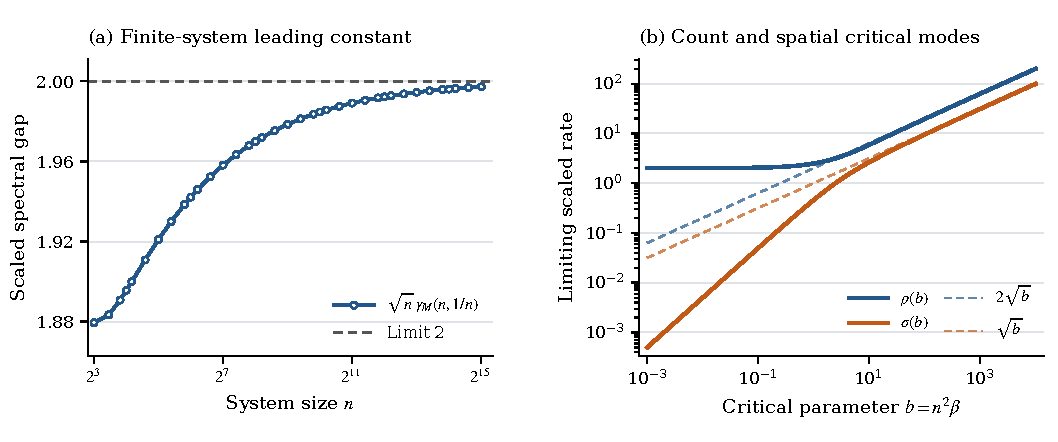
\includegraphics[width=\linewidth]{scaling_limits.pdf}
 \caption{Spectral scaling from finite radial matrices.
 (a) Direct numerical eigenvalues of the count derivative give
 $\sqrt n\,\gamma_M(n,1/n)$ approaching $2$.
 (b) Finite Jacobi approximations to $\rho(b)$ and $\sigma(b)$,
 with their large-$b$ equivalents $2\sqrt b$ and $\sqrt b$.
 The faint bands show the analytic truncation widths
 $2b/(R+3)$ and $b/(R+2)$, respectively, where
 $R=\lceil600(1+\sqrt b)\rceil$.
 Finite eigenvalues are evaluated in floating point; the bands do
 not include a certified rounding-error interval.
 Source data and the plotting program accompany the paper.}
 \label{fig:scaling-limits}
\end{figure}

\section{Total-variation and separation cutoff}\label{sec:count-cutoff}

For a finite chain with semigroup $P_t$ and stationary law $\pi$, write
\[
 d_x(t)=\|P_t(x,\cdot)-\pi\|_{\mathrm{TV}},\qquad
 d(t)=\max_x d_x(t),\qquad
 t_{\mathrm{mix}}(\varepsilon)=\inf\{t:d(t)\le\varepsilon\}.
\]
The superscripts ``count'' and ``polymer'' specify the chain. For a
specified initial state the maximum is omitted. All logarithms are
natural. The time-window statements below imply cutoff because the
window is smaller than the stated mixing time by a factor tending to
zero.

\subsection{The two polymer endpoints}
Let $L=L_M$ be the polymer generator, with stationary law $\pi=\pi_M$,
and write $K(x)$ for the number of polymers. The count strongly lumps
$L$ to the birth--death generator $Q$ on $\{1,\ldots,n\}$. Let $\bar\pi$ denote the pushforward of $\pi$ by $K$.
For every function $g$ on $\{1,\ldots,n\}$,
\[
 L(g\circ K)=(Qg)\circ K,
 \qquad P_t(g\circ K)=(\bar P_tg)\circ K.
\]
Fix $i$ such that the fiber $K^{-1}(i)$ consists of one state $x_i$.
The initial density with respect to stationarity is then
\[
 h_0(x)=\frac{\mathbf1_{\{x_i\}}(x)}{\pi(x_i)}
       =\frac{\mathbf1_{\{i\}}(K(x))}{\bar\pi(i)}.
\]
By reversibility, the density at time $t$ is $P_th_0$; invariance of the
count-function subspace gives
\[
 \frac{P_t(x_i,x)}{\pi(x)}
 =\frac{\bar P_t(i,K(x))}{\bar\pi(K(x))}.
\]
Consequently, at every $t\geq0$,
\[
 \boxed{\ \|P_t(x_i,\cdot)-\pi\|_{\rm TV}
       =\|\bar P_t(i,\cdot)-\bar\pi\|_{\rm TV}.\ }
\]
Indeed, sum the absolute density difference over each count fiber and use
$\sum_{K(x)=k}\pi(x)=\bar\pi(k)$. Both $i=1$ (one polymer of size $n$)
and $i=n$ (all monomers) have singleton fibers, so the identity holds at
both endpoints of the polymer chain. It transfers endpoint cutoff, and
provides a lower bound on worst-case polymer mixing. It does not provide
an upper bound for arbitrary initial polymer states.


\subsection{Count cutoff for fixed scaled fragmentation rate}
Throughout this section, $b>0$ is fixed and constants may depend on $b$.
Let $Q_n$ be the continuous-time birth--death generator on $\{1,\ldots,n\}$
with rates
\[
 \lambda_k=\frac{b(n-k)}n,\qquad \mu_k=\frac{k(k-1)}n.
\]
Its stationary law $p=p_n$ satisfies
\[
 p(k)\propto \binom nk\frac{b^k}{(k-1)!},\qquad
 \frac{p(k+1)}{p(k)}=\frac{b(n-k)}{k(k+1)}.
\]
Define the positive drift zero
\[
 a=a_n=\frac{-(b-1)+\sqrt{(b-1)^2+4bn}}2
       =\sqrt{bn}+O_b(1),
\]
so that
\[
 D_k:=\mu_k-\lambda_k
     =\frac{(k-a)(k+a+b-1)}n.
\]

\begin{theorem}[Count cutoff and polymer endpoint cutoff]\label{thm:count-cutoff}
For every fixed $b>0$, the count chains have a worst-case total-variation
cutoff at
\[
 t_n=\frac{\sqrt n\log n}{8\sqrt b}
\]
with an $O_b(\sqrt n)$ window. Precisely, for each $\varepsilon\in(0,1)$,
\[
 t^{\mathrm{count}}_{\mathrm{mix},n}(\varepsilon)
 =t_n+O_{b,\varepsilon}(\sqrt n).
\]
The same statement holds separately for the count chain started from $1$
and from $n$. The polymer chain at $\beta=b/n$ strongly lumps to $Q_n$. Its
total-variation distance from the single $n$-polymer and all-monomer states
equals the corresponding count distance at every time. These two polymer
initial states therefore have the same cutoff and window. In particular,
the worst-case polymer mixing time is at least
$t_n-O_{b,\varepsilon}(\sqrt n)$. An arbitrary-start upper bound is proved in
Theorem~\ref{thm:full-polymer-tv-upper-new}.
\end{theorem}

\subsection{Elementary stationary estimates}
Write $F_k=p([1,k])$ and $G_k=p([k,n])$. We shall use the following bounds:
\begin{align}
 \mathbb E_p|K-a|&\leq C_b\sqrt a,\label{eq:stationary-first-moment}\\
 c_{b,L}a^{-1/2}\leq p(k)&\leq C_{b,L}a^{-1/2}
       &&(|k-a|\leq L\sqrt a),\label{eq:stationary-local}\\
 F_k\wedge G_k&\geq c_{b,L}
       &&(|k-a|\leq L\sqrt a).\label{eq:stationary-central-masses}
\end{align}
Here $L$ is any fixed finite constant and $n$ is sufficiently large.
In particular every stationary median $m$ satisfies
$|m-a|\leq C_b\sqrt a$.

For completeness, these estimates follow directly from the consecutive
weight ratio. For unnormalized stationary weights $w_k$, set
\[
 R(x)=\frac{b(n-x)}{x(x+1)}.
\]
It is decreasing, and its unique positive solution to $R(x)=1$ is
$a+O_b(1)$. A maximizing index $r$ for $w_k$ therefore satisfies
$r=a+O_b(1)$. On $[a/2,2a]$, for all sufficiently large $n$,
\[
 -\frac{C_b}{a}\leq (\log R)'(x)
 =-\frac1{n-x}-\frac1x-\frac1{x+1}
 \leq-\frac{c_b}{a}.
\]
Since $R(r-1)\geq1\geq R(r)$, summing these derivative bounds over
successive ratios gives
\[
 c_b\exp\!\left(-C_b\frac{(k-a)^2}{a}\right)
 \leq\frac{w_k}{w_r}
 \leq C_b\exp\!\left(-c_b\frac{(k-a)^2}{a}\right),
 \qquad a/2\leq k\leq2a.
\]
Rounding endpoints changes only the constants. Below $a/2$, the successive
ratios in the direction away from the mode are bounded by a fixed number
$q_b<1$; the same holds above $2a$. These two tails are thus geometric,
starting at weights at most $C_be^{-c_ba}w_r$.
Consequently
\[
 \sum_k w_k\asymp_b\sqrt a\,w_r,\qquad
 \sum_k|k-a|w_k\leq C_b a\,w_r.
\]
This proves \eqref{eq:stationary-first-moment} and
\eqref{eq:stationary-local}. To obtain
\eqref{eq:stationary-central-masses}, sum the local lower bound over an
interval of length $\lfloor\sqrt a\rfloor$ immediately to the left, or
right, of $k$, using \eqref{eq:stationary-local} with $L+2$.
Finally, Markov's inequality applied to
\eqref{eq:stationary-first-moment} puts every median within
$C_b\sqrt a$ of $a$ (enlarging $C_b$ as needed).


\subsection{Endpoint hitting-time means}
Let $T_j$ be the first hitting time of $j$ and define the one-edge passage
means
\[
 e_k=\mathbb E_kT_{k+1}=\frac{F_k}{p(k)\lambda_k},\qquad
 f_k=\mathbb E_kT_{k-1}=\frac{G_k}{p(k)\mu_k}.
\]
These standard identities also follow by summing the Poisson equation
$Qh=-1$ against $p$ up to the absorbing edge. The recurrences are
\[
 \lambda_ke_k-\mu_ke_{k-1}=1,\qquad
 \mu_kf_k-\lambda_kf_{k+1}=1,
\]
with $e_1=1/\lambda_1$ and $f_n=1/\mu_n$.
Since $\lambda_k$ decreases and $\mu_k$ increases, induction in the first
recurrence shows that $e_k$ increases with $k$; reverse induction shows
that $f_k$ decreases with $k$.

Fix a stationary median $m$, and choose a fixed $L$ so large that
$|m-a|\leq(L-2)\sqrt a$. Put
$u=\lfloor a-L\sqrt a\rfloor$ and
$v=\lceil a+L\sqrt a\rceil$.
The stationary estimates imply, uniformly on the central interval
$[u,v]$,
\[
 e_k+f_k\leq C_{b,L}\sqrt a
\]
whenever the respective passage is defined: indeed
$p(k)\geq c_{b,L}/\sqrt a$ and
$\lambda_k\wedge\mu_k\geq c_b>0$ there. Hence all passages between
$u$, $m$, and $v$ together contribute $O_{b,L}(a)$ to their mean times.

For $k\leq u$ write $\delta_k=\lambda_k-\mu_k=-D_k>0$ and
$h_k=1/\delta_k$. The recurrence gives $e_k\leq h_k$ by induction, since
$h_k$ increases. If $\Delta_k=h_k-e_k$ and
$q_k=\mu_k/\lambda_k$, then
\[
 \Delta_1=0,\qquad
 \Delta_k=q_k\Delta_{k-1}+q_k(h_k-h_{k-1}).
\]
The sequence $q_k$ increases, and
\[
 h_k-h_{k-1}
 =\frac{2k+b-2}{n\delta_k\delta_{k-1}}
\]
also increases. Iterating and bounding the resulting geometric series
therefore gives
\[
 0\leq h_k-e_k
 \leq\frac{q_k}{1-q_k}(h_k-h_{k-1})
 \leq\frac{\mu_k(\delta_{k-1}-\delta_k)}{\delta_k^3}
 \leq\frac{C_ba^2}{(a-k)^3}.
\]
The last inequality uses $n\asymp_ba^2$, $\mu_k\leq C_b$,
$\delta_{k-1}-\delta_k\leq C_b/a$, and
$\delta_k\geq c_b(a-k)/a$. Summing for $k\leq u$ yields
\[
 \sum_{k=1}^{u}e_k
 =\sum_{k=1}^{u}\frac1{\delta_k}+O_{b,L}(a),
\]
because $\sum_{d\geq L\sqrt a-1}d^{-3}=O_L(a^{-1})$.

For $k\geq v$, put $h_k=1/D_k$. This time $h_k$ decreases, and
$h_k-h_{k+1}$ decreases as well: the function
$x\mapsto n/[x^2+(b-1)x-bn]$ is decreasing and convex for $x>a$
(and $n$ large). The ratio $p_k^*=\lambda_k/\mu_k$ decreases. Reverse
iteration of the recurrence, starting at $f_n=h_n$, gives
\[
 0\leq h_k-f_k
 \leq\frac{p_k^*}{1-p_k^*}(h_k-h_{k+1})
 \leq\frac{\lambda_k(D_{k+1}-D_k)}{D_k^3}
 \leq\frac{C_ba^2}{(k-a)^3}.
\]
At $k=n$ the difference is zero. For the final estimate, use
$\lambda_k\leq b$, $D_{k+1}-D_k=(2k+b)/n$, and
$D_k\geq c_b(k-a)(k+a)/n$; hence the displayed ratio is at most
$C_bn^2/[(k-a)^3(k+a)^2]\leq C_ba^2/(k-a)^3$.
It follows that
\[
 \sum_{k=v}^{n}f_k
 =\sum_{k=v}^{n}\frac1{D_k}+O_{b,L}(a).
\]

The reciprocal drift sums have elementary partial fractions:
\begin{align*}
 \sum_{k=1}^{u}\frac1{\delta_k}
 &=\frac n{2a+b-1}
   \sum_{k=1}^{u}\left(\frac1{a-k}+\frac1{a+k+b-1}\right),\\
 \sum_{k=v}^{n}\frac1{D_k}
 &=\frac n{2a+b-1}
   \sum_{k=v}^{n}\left(\frac1{k-a}-\frac1{k+a+b-1}\right).
\end{align*}
Integral comparison for the decreasing functions $1/x$ shows that each
bracketed sum is
$\tfrac12\log a+O_{b,L}(1)$: the first singular sum runs from a distance
of order $a$ down to $L\sqrt a$, and in the second sum the upper endpoint
contributes only
$\log[(n-a)/(n+a+b-1)]=O_b(a/n)$ after cancellation.
Thus, by the strong Markov property and addition of passage means,
\[
 \boxed{\begin{aligned}
 \mathbb E_iT_m
 &=\frac n{4a}\log a+O_b(a)\\
 &=\frac{\sqrt n\log n}{8\sqrt b}+O_b(\sqrt n),
 \qquad i\in\{1,n\}.
 \end{aligned}}
\]
More explicitly, both endpoint means separately equal the last expression.
The same proof works for any target $j$ with $|j-a|\leq L_0\sqrt a$,
with constants allowed to depend on the fixed $L_0$.


\subsection{Endpoint hitting-time variances}
Successive one-edge passage times are independent by the strong Markov
property. We prove
\[
 \operatorname{Var}_1T_m+\operatorname{Var}_nT_m=O_b(a^2)=O_b(n).
\]
For an upward passage $T=T_{k+1}$ started at $k$, let
$H(j)=\mathbb E_jT_{k+1}=\sum_{\ell=j}^{k}e_\ell$ for $j\leq k$.
The equations $QH=-1$ and
$Q\mathbb E_{\cdot}T_{k+1}^2=-2H$ on $\{1,\ldots,k\}$,
with zero boundary value at $k+1$, give upon summing against $p$
\begin{align*}
 \mathbb E_kT_{k+1}^2
 &=\frac2{p(k)\lambda_k}\sum_{j=1}^{k}p(j)H(j)\\
 &=\frac2{p(k)\lambda_k}\sum_{\ell=1}^{k}e_\ell F_\ell
 \leq2e_k^2\sum_{\ell=1}^{k}\frac{F_\ell}{F_k}.
\end{align*}
The inequality uses monotonicity of $e_\ell$ and
$e_k=F_k/[p(k)\lambda_k]$. In particular,
\begin{equation}\label{eq:upward-variance-bound}
 \operatorname{Var}_kT_{k+1}
 \leq2e_k^2\sum_{\ell=1}^{k}\frac{F_\ell}{F_k}.
\end{equation}
The reflected argument, using monotonicity of $f_k$, gives
\begin{equation}\label{eq:downward-variance-bound}
 \operatorname{Var}_kT_{k-1}
 \leq2f_k^2\sum_{\ell=k}^{n}\frac{G_\ell}{G_k}.
\end{equation}

For $k\leq u=\lfloor a-L\sqrt a\rfloor$, set
\[
 r_k=\frac{p(k-1)}{p(k)}
     =\frac{\mu_k}{\lambda_{k-1}}
     \leq\frac{\mu_k}{\lambda_k}<1,
\]
with $r_1=0$. These ratios increase with $k$. Shifting every index in
the sum defining $F_\ell$ by $k-\ell$ gives
$F_\ell\leq r_k^{k-\ell}F_k$. Consequently,
\[
 \sum_{\ell=1}^{k}\frac{F_\ell}{F_k}
 \leq\frac1{1-r_k}\leq\frac{\lambda_k}{\delta_k}.
\]
Together with $e_k\leq1/\delta_k$, this implies
\[
 \operatorname{Var}_kT_{k+1}
 \leq\frac{2\lambda_k}{\delta_k^3}
 \leq\frac{C_ba^3}{(a-k)^3}.
\]
Summing over $k\leq u$ gives $O_b(a^2)$.

For $k\geq v=\lceil a+L\sqrt a\rceil$, use instead the decreasing
ratios
\[
 s_k=\frac{p(k+1)}{p(k)}
     =\frac{\lambda_k}{\mu_{k+1}}
     \leq\frac{\lambda_k}{\mu_k}<1,
\]
with $s_n=0$. The same index-shifting argument gives
\[
 \sum_{\ell=k}^{n}\frac{G_\ell}{G_k}
 \leq\frac1{1-s_k}\leq\frac{\mu_k}{D_k}.
\]
Since $f_k\leq1/D_k$,
\[
 \operatorname{Var}_kT_{k-1}
 \leq\frac{2\mu_k}{D_k^3}.
\]
For $v\leq k\leq2a$, this is at most
$C_ba^3/(k-a)^3$, whose sum is $O_b(a^2)$.
For $k>2a$, use $D_k\geq c_bk^2/n$ and $\mu_k\leq k^2/n$
to obtain the bound $C_bn^2/k^4$; its sum is
$O_b(n^2/a^3)=O_b(a)$.

It remains to treat the $O_b(\sqrt a)$ central passages. Uniformly for
$k\in[u,v]$, the stationary estimates and the mean formulas give
$e_k+f_k\leq C_b\sqrt a$ and $F_k\wedge G_k\geq c_b>0$.
Furthermore,
\begin{align*}
 \sum_{\ell=1}^{k}F_\ell
 &=\mathbb E_p[(k-K+1)_+]\leq|k-a|+1+\mathbb E_p|K-a|
   \leq C_b\sqrt a,\\
 \sum_{\ell=k}^{n}G_\ell
 &=\mathbb E_p[(K-k+1)_+]\leq C_b\sqrt a.
\end{align*}
Equations \eqref{eq:upward-variance-bound} and
\eqref{eq:downward-variance-bound} therefore bound each central passage
variance by $C_ba^{3/2}$. Their total is $O_b(a^2)$.
Adding independent passage variances proves
\[
 \boxed{\quad
 \operatorname{Var}_1T_m\vee\operatorname{Var}_nT_m
 \leq C_ba^2\leq C_bn.
 \quad}
\]
As with the means, this bound remains valid for every target within a
fixed multiple of $\sqrt a$ of $a$, with the constant depending on that
multiple.


\subsection{Application of the birth--death cutoff theorem}
We use Chen--Saloff-Coste \cite[Theorem~1.4(1)]{CSC2015}.
In the continuous-time setting, if $m_n$ has
stationary mass bounded below on both sides, put
\[
 \theta_n=\max\{\mathbb E_1T_{m_n},\mathbb E_nT_{m_n}\},\qquad
 \alpha_n^2=\max\{\operatorname{Var}_1T_{m_n},
                         \operatorname{Var}_nT_{m_n}\}.
\]
Their theorem states that $\theta_n/\alpha_n\to\infty$ implies a
worst-case total-variation $(\theta_n,\alpha_n)$ cutoff. Its published
normalization starts from a stochastic matrix $B_n$ and uses the generator
$B_n-I$. To apply it here, take
\[
 c_n\geq\max_k(\lambda_k+\mu_k),\qquad B_n=I+Q_n/c_n.
\]
The continuous-time chain with generator $B_n-I$ is our chain slowed by
$c_n$. All passage means and standard deviations are multiplied by $c_n$;
both the criterion and its time-window conclusion therefore transfer
exactly to $Q_n$.

Take $m_n$ to be any stationary median. The previous two subsections give
\[
 \theta_n=t_n+O_b(a),\qquad \alpha_n=O_b(a),\qquad
 \frac{\theta_n}{\alpha_n}\longrightarrow\infty.
\]
The theorem yields
\[
 t^{\mathrm{count}}_{\mathrm{mix},n}(\varepsilon)
 =t_n+O_{b,\varepsilon}(a)
 =t_n+O_{b,\varepsilon}(\sqrt n).
\]
This proves the worst-case count assertion of
Theorem~\ref{thm:count-cutoff}.

To prove the assertion for each endpoint separately, it remains only to
give endpoint lower bounds; their upper bounds follow from the worst-case
bound. For a fixed $L>0$, let
$j_-=\lfloor a-L\sqrt a\rfloor$ and
$j_+=\lceil a+L\sqrt a\rceil$.
The stationary moment estimate gives
\[
 p([1,j_--1])\vee p([j_++1,n])\leq C_b/L.
\]
The preceding passage estimates, now with these central targets, give
\[
 \left|\mathbb E_1T_{j_-}-t_n\right|
 +\left|\mathbb E_nT_{j_+}-t_n\right|\leq C_{b,L}a,
 \qquad
 \operatorname{Var}_1T_{j_-}\vee\operatorname{Var}_nT_{j_+}
 \leq C_{b,L}a^2.
\]
By nearest-neighbor paths,
$\{T_{j_-}>t\}\subseteq\{K_t<j_-\}$ when $K_0=1$, and
$\{T_{j_+}>t\}\subseteq\{K_t>j_+\}$ when $K_0=n$.
Chebyshev's inequality therefore gives, for $A>C_{b,L}$ and $n$ large,
\[
 d_{n,1}(t_n-Aa)\wedge d_{n,n}(t_n-Aa)
 \geq1-\frac{C_b}{L}-\frac{C_{b,L}}{(A-C_{b,L})^2}.
\]
First choose $L$ and then $A$ large. Together with the count upper bound,
this proves both endpoint cutoffs with an $O_b(\sqrt n)$ window. The exact
endpoint identity in the first subsection completes the polymer endpoint
claims.

\subsection{A further consequence: separation cutoff}
Define separation from an initial state $x$ by
\[
 \operatorname{sep}_x(t)=1-\min_y\frac{P_t(x,y)}{\pi(y)}.
\]
The same established passage estimates give
\[
 s_n:=\mathbb E_1T_m+\mathbb E_nT_m
      =\frac{\sqrt n\log n}{4\sqrt b}+O_b(\sqrt n),\qquad
 v_n:=\sqrt{\operatorname{Var}_1T_m+\operatorname{Var}_nT_m}
      =O_b(\sqrt n).
\]
Chen--Saloff-Coste \cite[Theorem~1.3(1)]{CSC2015} implies endpoint separation cutoff at
$s_n$ with window $v_n$. In a continuous-time birth--death chain maximum
separation is attained from either boundary state; see their
Remark~1.2. Thus
\[
 t^{\mathrm{count}}_{\mathrm{sep},n}(\varepsilon)
 =\frac{\sqrt n\log n}{4\sqrt b}
       +O_{b,\varepsilon}(\sqrt n).
\]
The singleton-fiber identity gives a density that is constant on every
count fiber. Taking the minimum of that density, rather than summing its
absolute difference from one, proves the exact endpoint separation
identity for the polymer chain as well. Both polymer endpoint separation
mixing times therefore have this same asymptotic formula. This again does
not yield an arbitrary-start polymer upper bound.


\section{Mixing from an arbitrary polymer configuration}\label{sec:full-polymer-tv}
\begin{theorem}\label{thm:full-polymer-tv-upper-new}
For every fixed $b>0$, the polymer chain with $\beta=b/n$ satisfies
\[
 t^{\mathrm{polymer}}_{\mathrm{mix},n}(\varepsilon)
 \leq C_b\sqrt n\left\{(\log n)^2+\log(1/\varepsilon)\right\},
 \qquad 0<\varepsilon<1,
\]
for all sufficiently large $n$. Together with endpoint cutoff this gives,
for each fixed $\varepsilon\in(0,1)$,
\[
 \frac{\sqrt n\log n}{8\sqrt b}-O_{b,\varepsilon}(\sqrt n)
 \leq t^{\mathrm{polymer}}_{\mathrm{mix},n}(\varepsilon)
 \leq O_b\bigl(\sqrt n(\log n)^2\bigr).
\]
The extra logarithm in the upper bound is not removed by this argument;
worst-case polymer cutoff is not asserted.
\end{theorem}

\subsection{A degree-dependent sector bound}
Let $L_B$ be the labelled-cut comparison generator, and let
$\mathcal L_\ell$ be its degree-$\ell$ radial generator:
\begin{align*}
 (\mathcal L_\ell g)(k)
 ={}&\beta(n-k-\ell)(g(k+1)-g(k))\\
 &+\frac{(k-1)(k-\ell)}n(g(k-1)-g(k))
 -\left(\ell\beta+\frac{\ell(k-1)}n\right)g(k),
 \qquad \ell\leq k\leq n-\ell.
\end{align*}
Assume $2\leq A:=n\sqrt\beta\leq n/4$. For $\ell\geq1$ use
\[
 h_\ell(k)=\frac1{(k+A)_\ell},\qquad
 (x)_\ell=x(x+1)\cdots(x+\ell-1).
\]
Its neighboring ratios are
\[
 \frac{h_\ell(k+1)}{h_\ell(k)}=\frac{k+A}{k+A+\ell},\qquad
 \frac{h_\ell(k-1)}{h_\ell(k)}=\frac{k+A+\ell-1}{k+A-1}.
\]
Direct substitution gives the exact identity
\begin{equation}\label{eq:degree-certificate-new}
 \frac{-(\mathcal L_\ell h_\ell)(k)}{h_\ell(k)}
 =\ell\left[
 \frac{\beta(n-k-\ell)}{k+A+\ell}+\beta
 +\frac{(k-1)(A+\ell-1)}{n(k+A-1)}\right].
\end{equation}
All bracketed terms are nonnegative. If $k\leq A$, then $\ell\leq k$
gives $n-k-\ell\geq n/2$ and $k+A+\ell\leq3A$; the first term is
at least $\sqrt\beta/6$. If $k\geq A$, then
\[
 \frac{k-1}{k+A-1}\geq\frac13,\qquad A+\ell-1\geq A,
\]
so the last term is at least $\sqrt\beta/3$.
The finite positive-vector comparison therefore proves that every
eigenvalue in degree $\ell$ is at least
\begin{equation}\label{eq:degree-linear-lower-new}
 \lambda_\ell\geq\frac{\ell\sqrt\beta}{6}.
\end{equation}
Independently, the killing term gives
\[
 \lambda_\ell\geq\ell\beta+\frac{\ell(\ell-1)}n.
\]
In particular, at fixed $b>0$, $\beta=b/n$, and $A=\sqrt{bn}$,
\[
 \lambda_\ell\geq \frac{b\ell}{6A}
 \qquad(1\leq\ell\leq\lfloor n/2\rfloor)
\]
for every sufficiently large $n$.


\subsection{A polynomial bound on the count density}
Fix $b>0$, put $A=\sqrt{bn}$, and let $p$ be the stationary count law.
Let $r$ be a mode of $p$ and define
\[
 V(k)=\left(\frac{p(r)}{p(k)}\right)^{3/4}\geq1,
 \qquad W(k)=(\sqrt{\lambda_k}-\sqrt{\mu_k})^2.
\]
We prove the drift inequality
\begin{equation}\label{eq:count-log-lyapunov-new}
 \frac{(QV)(k)}{V(k)}
 \leq\frac{C_b-c_b\log V(k)}{A},\qquad 1\leq k\leq n,
\end{equation}
for all sufficiently large $n$.

By detailed balance, the exact expression is
\[
 \frac{QV(k)}{V(k)}
 =\lambda_k^{1/4}\mu_{k+1}^{3/4}
  +\mu_k^{1/4}\lambda_{k-1}^{3/4}-\lambda_k-\mu_k.
\]
At an endpoint the term with zero outgoing rate is zero; thus the displayed
formula remains valid if one formally sets $\lambda_0=b$ and
$\mu_{n+1}=n+1$. These are algebraic conventions only.
Write $\lambda=\lambda_k$ and $\mu=\mu_k$. With
$u=\lambda^{1/4}$ and $v=\mu^{1/4}$,
\begin{align*}
 &\lambda+\mu-\lambda^{1/4}\mu^{3/4}-\mu^{1/4}\lambda^{3/4}\\
 &\hspace{1cm}=(u-v)^2(u^2+uv+v^2)
 \geq\frac34(u-v)^2(u+v)^2
 =\frac34W(k).
\end{align*}
The two coefficient-variation errors are
\[
 E_1=\lambda_k^{1/4}(\mu_{k+1}^{3/4}-\mu_k^{3/4}),\qquad
 E_2=\mu_k^{1/4}(\lambda_{k-1}^{3/4}-\lambda_k^{3/4}).
\]
Since $\mu_{k+1}-\mu_k=2k/n$, concavity gives, for $k\geq2$,
\[
 E_1\leq\frac34\lambda_k^{1/4}\mu_k^{-1/4}\frac{2k}{n}
       \leq C_b n^{-3/4}\sqrt k.
\]
The same bound holds at $k=1$ by direct substitution, since
$E_1=\lambda_1^{1/4}(2/n)^{3/4}$.
For $k\leq2A$, it follows that $E_1\leq C_b/A$.
For $k>2A$, one has $\mu_k\geq3b\geq3\lambda_k$ and hence
$W(k)\geq c_bk^2/n$ (for large $n$). Thus
\[
 \frac{E_1}{W(k)}\leq C_bn^{1/4}k^{-3/2}\leq\frac{C_b}{A}.
\]
For sufficiently large $n$, this is at most $1/4$.
The inequality $(x+y)^{3/4}-x^{3/4}\leq y^{3/4}$ also gives, uniformly
including $k=n$,
\[
 E_2\leq\mu_k^{1/4}(b/n)^{3/4}
 \leq\frac{b^{3/4}\sqrt k}{n}\leq\frac{C_b}{A}.
\]
Consequently
\begin{equation}\label{eq:count-drift-square-new}
 \frac{QV(k)}{V(k)}\leq-\frac12W(k)+\frac{C_b}{A}.
\end{equation}

It remains to check
\begin{equation}\label{eq:stationary-weight-vs-drift-new}
 \log V(k)\leq C_b\{1+A W(k)\}.
\end{equation}
On $A/2\leq k\leq2A$, the elementary stationary ratio estimates proved
earlier give
\[
 \log\frac{p(r)}{p(k)}\leq C_b\left(1+\frac{(k-A)^2}{A}\right).
\]
The exact drift factorization around its zero $a=A+O_b(1)$ and
$\lambda_k+\mu_k\leq C_b$ give
$W(k)\geq c_b(k-a)^2/A^2$, proving
\eqref{eq:stationary-weight-vs-drift-new} on this interval.
If $k<A/2$, then $W(k)\geq c_b>0$, while
\[
 \log\frac{p(r)}{p(k)}\leq\log\frac{p(r)}{p(1)}
 \leq\log\frac{A^{2(r-1)}}{(r-1)!\,r!}\leq C_bA,
\]
where $r=A+O_b(1)$ and the last bound follows from
$j!\geq(j/e)^j$.
If $k>2A$, sum the consecutive ratios to obtain
\[
 \log\frac{p(r)}{p(k)}
 =\sum_{j=r}^{k-1}
 \left[\log\frac jA+\log\frac{j+1}A-\log(1-j/n)\right]
 \leq\frac{C_bk^2}{A}.
\]
Here $\log x\leq x$ controls the first two terms. For the last,
$-\log(1-j/n)\leq2j/n$ when $k\leq n/2$; when $k>n/2$, its sum is
at most
$\sum_{j=1}^{n-1}-\log(1-j/n)\leq Cn\leq Ck^2/n$.
Since $W(k)\geq c_bk^2/n$ and $A^2=bn$, this proves
\eqref{eq:stationary-weight-vs-drift-new} in the remaining case.
Combining it with \eqref{eq:count-drift-square-new} proves
\eqref{eq:count-log-lyapunov-new}.

Now let $y(t)=\mathbb E_iV(K_t)$ for any initial count $i$.
The finite-state evolution equation and Jensen's inequality for
$x\log x$ imply
\[
 y'(t)\leq\frac{C_b}{A}y(t)-\frac{c_b}{A}y(t)\log y(t).
\]
Thus $z(t)=\log y(t)$ satisfies
\[
 z(t)\leq\frac{C_b}{c_b}+e^{-c_bt/A}z(0).
\]
Uniformly in $i$, \eqref{eq:stationary-weight-vs-drift-new} and
$W(i)\leq\lambda_i+\mu_i\leq b+n$ give
$z(0)\leq C_bn^2$. Consequently there exists $C_b<\infty$ such that
\begin{equation}\label{eq:count-V-moment-new}
 \sup_i\sup_{t\geq t_0}\mathbb E_iV(K_t)\leq C_b,
 \qquad t_0=C_b A\log n.
\end{equation}

Let $q_t$ be any count distribution at time $t\geq t_0$ started from a
point mass (or any mixture). Equation \eqref{eq:count-V-moment-new}
gives $q_t(k)\leq C_b/V(k)$. The stationary Gaussian and geometric-tail
estimates give
\[
 p(r)\asymp_b A^{-1/2},\qquad \sum_k\sqrt{p(k)}\leq C_b A^{1/4}.
\]
It follows that
\begin{equation}\label{eq:count-L2-polynomial-new}
 M(t):=\sum_{k=1}^n\frac{q_t(k)^2}{p(k)}
 \leq C_bp(r)^{-3/2}\sum_k\sqrt{p(k)}\leq C_bA,
 \qquad t\geq t_0.
\end{equation}
This is a polynomial bound, not a claim that count $L^2$ mixing is complete.


\subsection{The polymer mixing bound}


Let $p_{\mathrm{cut}}$ be the map from nonempty labelled cut sets to their
unordered segment lengths, and write $\pi_B$, $\pi_M$, and $p$ for the
stationary cut, polymer, and count laws, respectively. Start the actual
polymer chain from any state $x$. Let $f_t$ be its density with respect to
$\pi_M$, and lift it by
\[
 F_t(S)=f_t(p_{\mathrm{cut}}(S)).
\]
The lift is nonnegative. Its average on the layer $|S|=k$ is
\[
 \overline F_t(k)=\frac{q_t(k)}{p(k)},
\]
where $q_t$ is the distribution of the actual polymer count. Strong
lumpability of the count means that $q_t$ evolves under $Q$ from $K(x)$.
The preceding Lyapunov calculation therefore gives, with $A=\sqrt{bn}$,
\begin{equation}\label{eq:polymer-count-warm-new}
 M(t):=\sum_kp(k)\overline F_t(k)^2\leq M_*:=C_bA,
 \qquad t\geq t_0:=C_bA\log n.
\end{equation}
Choose the constant so that $M_*\geq1$.

Let $P_\ell$ denote the orthogonal projection onto the complete
degree-$\ell$ sector of the labelled-cut comparison space, and set
\[
 d_\ell=\dim H_\ell=\binom n\ell-\binom n{\ell-1}.
\]
On a layer of size $N_k=\binom nk$, the projector onto degree $\ell$
has constant diagonal $d_\ell/N_k$ whenever that degree is present.
Indeed, the projector commutes with every permutation of the labels,
and its trace is $d_\ell$. Positive semidefiniteness then gives
\[
 |P_\ell(S,T)|\leq\sqrt{P_\ell(S,S)P_\ell(T,T)}=d_\ell/N_k.
\]
For every nonnegative function $F$, it follows, using the ordinary matrix
kernel of this layerwise projector, that
\begin{align*}
 \|P_\ell F\|_{L^2(\pi_B)}^2
 &=\sum_k\frac{p(k)}{N_k}
       \sum_{|S|=|T|=k}F(S)P_\ell(S,T)F(T)\\
 &\leq d_\ell\sum_kp(k)\overline F(k)^2.
\end{align*}
Absent degrees contribute zero. Telescoping the dimensions gives
\begin{equation}\label{eq:positive-low-degree-new}
 \sum_{\ell=0}^{d}\|P_\ell F_t\|_2^2
 \leq\binom nd M(t),\qquad 0\leq d\leq\lfloor n/2\rfloor.
\end{equation}

Put $R(t)=\|F_t\|_{L^2(\pi_B)}^2=\|f_t\|_{L^2(\pi_M)}^2$ and
$g=\sqrt\beta/6=b/(6A)$. The stationary Dirichlet-form identity and
the proved sector bound $\lambda_\ell\geq g\ell$ imply
\begin{align*}
 -R'(t)
 &=2\mathcal E_M(f_t,f_t)=2\mathcal E_B(F_t,F_t)\\
 &\geq2g(d+1)\sum_{\ell>d}\|P_\ell F_t\|_2^2\\
 &\geq2g(d+1)\left\{R(t)-M_*\binom nd\right\},
 \qquad t\geq t_0.
\end{align*}
This is a statement about the actual polymer evolution; no invariance of
the polymer lift under the cut semigroup, or under individual sector
projections, is assumed. The sector decomposition is used only to bound
the instantaneous stationary energy.

Positivity also bounds the initial size of this differential inequality:
on each layer, $\sum_SF_t(S)^2\leq(\sum_SF_t(S))^2$, so
\[
 R(t)\leq\sum_kp(k)\binom nk\overline F_t(k)^2
       \leq2^nM_*,\qquad t\geq t_0.
\]
For $n$ large, whenever $R(t)>16M_*n^2$, put
\[
 s(t)=\log\frac{R(t)}{M_*},\qquad
 d=\left\lfloor\frac{s(t)}{2\log n}\right\rfloor.
\]
Then $1\leq d<\lfloor n/2\rfloor$, because
$s(t)\leq n\log2$. Moreover,
\[
 M_*\binom nd\leq M_*n^d\leq M_*e^{s(t)/2}\leq R(t)/4.
\]
The energy inequality consequently gives
\[
 s'(t)=\frac{R'(t)}{R(t)}
 \leq-g(d+1)\leq-\frac{g}{2\log n}s(t).
\]
Since $s(t_0)\leq n\log2$, it takes at most
$2g^{-1}(\log n)^2$ additional time to reach
$R(t)\leq16M_*n^2$. Once this threshold is reached it remains satisfied,
because $R(t)$ is nonincreasing.

Finally use the already established polymer gap
$\gamma_M\geq c_b/A$. If $t_1$ is the preceding threshold time, then
\[
 R(t_1+u)-1\leq e^{-2\gamma_Mu}\{R(t_1)-1\},\qquad
 \|P^M_{t_1+u}(x,\cdot)-\pi_M\|_{\rm TV}
 \leq\frac12\sqrt{R(t_1+u)-1}.
\]
As $R(t_1)\leq16C_bAn^2$, an additional
$C_bA\{\log n+\log(1/\varepsilon)\}$ time suffices. This proves
Theorem~\ref{thm:full-polymer-tv-upper-new}, uniformly over the initial
polymer state $x$.

\section{Cut reactions with graph diffusion}
\label{sec:spatial-diffusion}

Let $G=(V,E,c)$ be a connected weighted graph on $n\geq2$ vertices,
with symmetric nonnegative edge weights $c_{xy}$.  Its random-walk
Laplacian is
\[
 (\Delta_G a)(x)=\sum_yc_{xy}[a(x)-a(y)],
\]
and $\lambda_G>0$ denotes its smallest eigenvalue on the mean-zero
subspace.  On the nonempty subsets of $V$, define
\begin{equation}\label{eq:spatial-generator}
 \begin{split}
 (\mathcal L_{\beta,D,G}f)(S)
 ={}&\beta\sum_{x\notin S}[f(S\cup\{x\})-f(S)]\\
 &+\frac{|S|-1}{n}\sum_{x\in S}[f(S\setminus\{x\})-f(S)]\\
 &+D\sum_{\{x,y\}\in E}c_{xy}[f(S^{xy})-f(S)],
 \qquad \beta>0,\quad D\geq0,
 \end{split}
\end{equation}
where $S^{xy}$ exchanges the occupancy of $x$ and $y$.  The deletion
sum is zero at $|S|=1$.  The first two terms are the cut-reaction
generator, and the last term is conservative exclusion along $G$.
The reversible probability measure remains
\begin{equation}\label{eq:spatial-reversible-law}
 \pi_\beta(S)=Z^{-1}\frac{(\beta n)^{|S|}}{(|S|-1)!}.
\end{equation}
Indeed, its adjacent-cardinality weights satisfy detailed balance for
the reaction rates, and it is invariant under every coordinate
permutation.

The cardinality is the birth--death chain with rates
$\beta(n-k)$ and $k(k-1)/n$; write $\gamma_Q(n,\beta)$ for its gap.
The degree-one radial reaction operator acts on $k=1,\ldots,n-1$ as
\begin{equation}\label{eq:spatial-degree-one}
 \begin{split}
 (A_1h)(k)
 ={}&\beta(n-k-1)[h(k+1)-h(k)]\\
 &+\frac{(k-1)^2}{n}[h(k-1)-h(k)]
   -\left(\beta+\frac{k-1}{n}\right)h(k).
 \end{split}
\end{equation}
Let $\eta_1(n,\beta)$ be the smallest eigenvalue of $-A_1$.

\begin{theorem}[Exact gap with graph diffusion]
\label{thm:spatial-exact-gap}\label{thm:spatial-gap}
For every $n,\beta,D,G$ as above, the spectral gap of
\eqref{eq:spatial-generator} is
\begin{equation}\label{eq:spatial-exact-gap}
 \gamma_{\mathrm{sp}}(n,\beta,D,G)
 =\min\{\gamma_Q(n,\beta),\ \eta_1(n,\beta)+D\lambda_G\}.
\end{equation}
\end{theorem}

\begin{proof}
Use the Boolean harmonic decomposition of the cut chain.  In degree
$\ell$, functions are sums of products $h(|S|)H(S)$, where $H$ belongs
to the degree-$\ell$ harmonic space and $h$ is supported on the
allowable cardinalities.  The reaction generator acts on this sector
as $A_\ell\otimes I$, where $A_\ell=\mathcal L_\ell$.  Every coordinate permutation preserves harmonic
degree and commutes with the canonical lifts between slices.  Hence
the graph-swap generator acts as $I\otimes\mathcal S_{G,\ell}$, with
the same harmonic action at every cardinality.  The slice inner
products on the harmonic factor differ only by a scalar, so these
are tensor decompositions of the reversible Hilbert spaces as well.
Consequently the generator on the degree-$\ell$ sector is
\begin{equation}\label{eq:spatial-tensor-sum}
 A_\ell\otimes I+I\otimes D\mathcal S_{G,\ell}.
\end{equation}
The negative of the graph-swap operator is nonnegative, since it is
the restriction of a reversible Markov generator with its sign
changed.

In degree zero, swaps act trivially and the first positive eigenvalue
is $\gamma_Q$.  In every degree $\ell\geq2$,
Proposition~\ref{prop:higher-exact} gives
$\inf\operatorname{Spec}(-A_\ell)\geq\gamma_Q$; adding the graph form
cannot lower this bound.

For degree one write
\[
 H_a(S)=\sum_{x\in S}a(x),\qquad \sum_{x\in V}a(x)=0.
\]
A direct calculation gives
$\mathcal S_G H_a=-H_{\Delta_Ga}$.  Thus the degree-one eigenvalues
are sums of eigenvalues of $-A_1$ and of $D\Delta_G$ on mean-zero
vectors.  Their smallest value is $\eta_1+D\lambda_G$.  Taking the
minimum over all degrees proves~\eqref{eq:spatial-exact-gap}.
\end{proof}

Only the one-particle graph action is required in this proof.  Higher
harmonic sectors already lie above the count gap before diffusion is
added.

\begin{proposition}[An additive-error formula for the degree-one gap]
\label{prop:spatial-degree-one-sharp}
Set
\[
 d=\sqrt{\beta^2+4\beta},\qquad
 c_1=\frac{\beta+d}{2},\qquad a=nc_1.
\]
Then
\begin{equation}\label{eq:spatial-degree-one-endpoint-bracket}
 c_1-\frac{2a}{n(a+2)}
 \leq\eta_1(n,\beta)
 \leq c_1-\frac{2a^2}{n(n+a-2)(n+a)}.
\end{equation}
In particular,
\begin{equation}\label{eq:spatial-degree-one-additive-error}
 c_1-\frac2n\leq\eta_1(n,\beta)\leq c_1.
\end{equation}
\end{proposition}

\begin{proof}
The number $a$ is positive and satisfies $a^2=\beta n(n+a)$.
For $h(k)=1/(k+a)$ the quotient in
\eqref{eq:spatial-reciprocal-quotient} simplifies to
\begin{equation}\label{eq:spatial-sharp-reciprocal-quotient}
 -\frac{A_1h(k)}{h(k)}
 =\frac an-\frac{2a^2}{n(k+a-1)(k+a+1)}.
\end{equation}
Every denominator is positive, even when $a<1$, since $k\geq1$.
The quotient increases with $k$.  Its values at $k=1$ and $k=n-1$
give~\eqref{eq:spatial-degree-one-endpoint-bracket} by positive-vector
comparison.  The simpler bracket follows from $a/(a+2)\leq1$.
\end{proof}

\begin{corollary}[Leading constants with graph diffusion]
\label{cor:spatial-leading-constants}
With $d$ and $c_1$ as above, put
\[
 m=\min\{d,c_1+D\lambda_G\}.
\]
The count-chain bracket $d-5/n\leq\gamma_Q\leq d+4/n$ from
Theorem~\ref{thm:sharp-gap} and
Theorem~\ref{thm:spatial-exact-gap} imply
\begin{equation}\label{eq:spatial-leading-constants}
 m-\frac5n\leq\gamma_{\mathrm{sp}}(n,\beta,D,G)
 \leq m+\frac4n.
\end{equation}
In particular, if $n^2\beta\longrightarrow\infty$, the ratio of
$\gamma_{\mathrm{sp}}$ to $m$ tends to one, uniformly in the graph
and in $D\geq0$.
\end{corollary}

\begin{proof}
Combine Theorem~\ref{thm:sharp-gap} and the degree-one additive-error
bracket inside the minimum in
\eqref{eq:spatial-exact-gap}.  For the final assertion, observe that
$d\geq2\sqrt\beta$ and $c_1\geq\sqrt\beta$, so
$nm\geq n\sqrt\beta\longrightarrow\infty$.
\end{proof}

\begin{proposition}[The degree-one scale]
\label{prop:spatial-degree-one-scale}
For every $n\geq2$ and $\beta>0$, set
\[
 u=\beta+\min\{n\beta,\sqrt\beta\}.
\]
Then
\begin{equation}\label{eq:spatial-degree-one-scale}
 \frac u8\leq\eta_1(n,\beta)\leq u.
\end{equation}
More precisely, with $c_0=1-2^{-1/2}$,
\begin{equation}\label{eq:spatial-degree-one-auxiliary}
 \max\left\{\beta,\min\left(c_0n\beta,\frac1{2n}\right)\right\}
 \leq\eta_1
 \leq\min\left\{\frac{n\beta}{2},\beta+\sqrt\beta\right\}.
\end{equation}
Also,
\begin{equation}\label{eq:spatial-degree-one-below-count}
 \eta_1\leq\gamma_Q-\frac2n.
\end{equation}
In particular, the gap of the cut-reaction chain without graph
diffusion is exactly $\eta_1$.
\end{proposition}

\begin{proof}
The positive test function $h(k)=1/k$ gives the exact quotient
\[
 -\frac{A_1h(k)}{h(k)}=\frac{\beta n}{k+1}\leq\frac{n\beta}{2},
\]
which proves the first upper bound.  For the second, put $j=k-1$ and
consider the conservative part of $A_1$.  Its birth rate is
$\beta(n-2-j)$, its death rate is $j^2/n$, and its killing is
$\beta+j/n$.  If $\nu$ is the invariant law of this finite
conservative chain, stationarity applied to $j$ yields
\[
 \mathbb E_\nu j^2
 =\beta n(n-2-\mathbb E_\nu j)\leq\beta n^2.
\]
The constant-function Rayleigh quotient, followed by Cauchy--Schwarz,
therefore gives $\eta_1\leq\beta+\sqrt\beta$.  When $n=2$ the
conservative chain has the single state $j=0$, so the same argument
applies.

The killing term gives $\eta_1\geq\beta$.  For another lower bound
use $h(k)=k^{-1/2}$.  At $k=1$ its quotient is
\[
 \beta+\beta(n-2)(1-2^{-1/2})\geq c_0n\beta.
\]
For $k\geq2$, discard the nonnegative birth term and the term $\beta$
to obtain
\[
 -\frac{A_1h(k)}{h(k)}
 \geq\frac{k-1}{n}
 \left[1-(k-1)\left(\sqrt{\frac{k}{k-1}}-1\right)\right]
 \geq\frac1{2n}.
\]
Here
$(k-1)(\sqrt{k/(k-1)}-1)=1/(\sqrt{k/(k-1)}+1)\leq1/2$.
Positive-vector comparison proves
\eqref{eq:spatial-degree-one-auxiliary}.

It remains to obtain a square-root lower bound in the intermediate
range.  If $n\geq8$ and $4/n^2\leq\beta\leq1/16$, put
$a=n\sqrt\beta$, so that $2\leq a\leq n/4$, and use
$h(k)=1/(k+a)$.  Direct cancellation gives
\begin{equation}\label{eq:spatial-reciprocal-quotient}
 -\frac{A_1h(k)}{h(k)}
 =\beta+\frac{\beta(n-k-1)}{k+a+1}
       +\frac{a(k-1)}{n(k+a-1)}.
\end{equation}
If $k\leq a$, then $n-k-1\geq n/2$ and $k+a+1\leq5a/2$,
so the second term is at least $\sqrt\beta/5$.  If $k\geq a$,
then $k-1\geq k/2$ and $k+a-1\leq2k$, so the final term is at
least $\sqrt\beta/4$.  Thus $\eta_1\geq\sqrt\beta/5$ in this
range.

The estimates patch with a universal constant.  For
$\beta\leq n^{-2}$, the lower bound $c_0n\beta$ is at least
$(n+1)\beta/8=u/8$.  For $n\leq7$ and $\beta\geq n^{-2}$,
$u\leq8\beta$.  If $n\geq8$ and
$n^{-2}\leq\beta\leq4n^{-2}$, the auxiliary bound is at least
$c_0/n\geq\sqrt\beta/7$; combine this with $\eta_1\geq\beta$.
In the intermediate range just treated the two lower bounds give
$u\leq6\eta_1$.  Finally, for $\beta\geq1/16$, $u\leq5\beta$.
These cases prove the lower bound in~\eqref{eq:spatial-degree-one-scale}.
The two upper bounds in~\eqref{eq:spatial-degree-one-auxiliary}
immediately give $\eta_1\leq u$.

Finally, let $h$ be the positive ground state of the count-derivative
operator $A_{n,\beta}$.  Its forward ratios are at least $1/2$ by
Lemma~\ref{lem:critical-ground-ratios} (or by the weaker ratio bound
used in Proposition~\ref{prop:higher-exact}).  Direct subtraction gives
\[
 \frac{(A_{n,\beta}-A_1)h(k)}{h(k)}
 =\frac{(k-1)h(k-1)/h(k)-2k}{n}\leq-\frac2n.
\]
At $k=1$ the backward term is zero.  Testing $-A_1$ with $h$ proves
\eqref{eq:spatial-degree-one-below-count}, and
Theorem~\ref{thm:spatial-exact-gap} gives the last assertion.
\end{proof}

\begin{corollary}[A uniform spatial phase diagram]
\label{cor:spatial-uniform-gap}
Put $s=\beta+\sqrt\beta+n^{-1}$ and
$u=\beta+\min\{n\beta,\sqrt\beta\}$.  Then
\begin{equation}\label{eq:spatial-uniform-gap}
 \frac18\min\{s,u+D\lambda_G\}
 \leq\gamma_{\mathrm{sp}}(n,\beta,D,G)
 \leq4\min\{s,u+D\lambda_G\}.
\end{equation}
In particular, for $0<\beta\leq n^{-2}$,
\begin{equation}\label{eq:spatial-rare-gap}
 \gamma_{\mathrm{sp}}(n,\beta,D,G)
 \asymp\min\{n^{-1},n\beta+D\lambda_G\},
\end{equation}
with absolute comparison constants.
\end{corollary}

\begin{proof}
Combine Theorem~\ref{thm:spatial-exact-gap} and
Proposition~\ref{prop:spatial-degree-one-scale} with the count-chain
bounds $s/6\leq\gamma_Q\leq4s$.  In the stated rare-fragmentation
range, $s\asymp n^{-1}$ and $u\asymp n\beta$.
\end{proof}

For a unit-rate cycle on $n\geq3$ vertices,
$\lambda_G=4\sin^2(\pi/n)$.  For the discrete torus of side
$L\geq3$ in dimension $d$, with unit rates along its edges,
$n=L^d$ and $\lambda_G=4\sin^2(\pi/L)$.  Thus
\eqref{eq:spatial-rare-gap} becomes
\[
 \gamma_{\mathrm{sp}}
 \asymp\min\{n^{-1},n\beta+D/L^2\}
\]
on a torus.  This identifies the competition between count relaxation,
reactions that renew a dilute cut configuration, and graph diffusion.

On a cycle, adding or deleting a cut splits or merges neighboring
intervals, and exchanging adjacent occupied and unoccupied vertices
moves an interval boundary.  On a general graph,
\eqref{eq:spatial-generator} is an exclusion process with
cardinality-dependent creation and deletion.  Its reaction rates
retain the global count dependence and its equilibrium law remains
exchangeable.  These features permit the tensor decomposition and
specify the scope of the spatial result.

\subsection{Inhomogeneous reversible reactions}

The exact formula also controls reaction rates that depend on the
positions and surrounding configuration, through a comparison of
reversible conductances.  For each undirected reaction edge
$e=\{S,S\cup\{x\}\}$ with $S\neq\varnothing$ and $x\notin S$,
choose a factor $a_e$ satisfying
\[
 0<a_-\leq a_e\leq a_+<\infty.
\]
Multiply both the addition rate from $S$ to $S\cup\{x\}$ and the
reverse deletion rate by this same factor.  Keep the graph-swap
generator and its diffusion coefficient $D$ unchanged.  Write
$\gamma_{\mathrm{inhom}}$ for the resulting gap.

\begin{corollary}[Bounded inhomogeneous reaction rates]
\label{cor:spatial-inhomogeneous}
The modified chain is reversible for~\eqref{eq:spatial-reversible-law}
and satisfies
\begin{equation}\label{eq:spatial-inhomogeneous-gap}
 \begin{split}
 \min\{a_-\gamma_Q,\ a_-\eta_1+D\lambda_G\}
 &\leq\gamma_{\mathrm{inhom}}\\
 &\leq\min\{a_+\gamma_Q,\ a_+\eta_1+D\lambda_G\}.
 \end{split}
\end{equation}
The factors may depend arbitrarily on the edge and its configuration;
the modified reaction generator need not commute with permutations.
\end{corollary}

\begin{proof}
Multiplication by the same factor in both directions preserves
detailed balance at each reaction edge.  Let $\mathcal E_B$ be the
reaction form and $\mathcal E_G$ the unit-diffusion graph-swap form,
both with respect to $\pi_\beta$.  The modified form satisfies
\[
 a_-\mathcal E_B(f,f)+D\mathcal E_G(f,f)
 \leq\mathcal E_{\mathrm{inhom}}(f,f)
 \leq a_+\mathcal E_B(f,f)+D\mathcal E_G(f,f).
\]
For any constant $a>0$, Theorem~\ref{thm:spatial-exact-gap}, with
diffusion coefficient $D/a$ and then a change of time by $a$, gives
the gap of $aB+D\mathcal S_G$ as
$\min\{a\gamma_Q,a\eta_1+D\lambda_G\}$.  All three forms have the
same variance denominator.  Taking their infima proves
\eqref{eq:spatial-inhomogeneous-gap}.
\end{proof}

For example, place the vertices in a cyclic order and let adding a
cut at $x$ divide an interval into two positive lengths $i$ and $j$.
For $|\varepsilon|<1/2$, set
\begin{equation}\label{eq:spatial-circle-inhomogeneity}
 a_{\{S,S\cup\{x\}\}}
 =1+\varepsilon\cos\left(\frac{2\pi x}{n}\right)
   +\varepsilon\frac{(i-j)^2}{(i+j)^2}.
\end{equation}
This combines a spatially varying environment with a dependence on
the neighboring interval lengths.  The factor is unchanged when
$i$ and $j$ are interchanged, and the same split determines it for
the reverse merger.  It satisfies
$1-2|\varepsilon|\leq a_e\leq1+2|\varepsilon|$, so
Corollary~\ref{cor:spatial-inhomogeneous} applies with these constants.
The corollary covers bounded reversible modifications of the stated
reaction edges; its proof does not extend the exact formula to
arbitrary coagulation or fragmentation kernels.

\section{Nonreversible conservative motion of cuts}
\label{sec:nonreversible}

The reduction in Theorem~\ref{thm:spatial-gap} extends to conservative
jumps that permute the sites, without requiring inverse jumps to have
the same rate.  The state in this section is the full nonempty cut set.
As in the spatial model, unordered interval lengths need not form a
Markov process.

For $\sigma\in S_n$ put $(T_\sigma F)(S)=F(\sigma S)$, and let
\begin{equation}\label{eq:permutation-motion}
 H=\sum_{\sigma\in S_n}r_\sigma(T_\sigma-I),
 \qquad r_\sigma\ge0,\qquad
 L=L_B+DH,\quad D\ge0.
\end{equation}
Terms with $r_\sigma=0$ may be omitted.  No relation between
$r_\sigma$ and $r_{\sigma^{-1}}$ is imposed.
The induced one-coordinate generator is
\begin{equation}\label{eq:one-coordinate-motion}
 (H_1a)(x)=\sum_\sigma r_\sigma\bigl(a(\sigma x)-a(x)\bigr).
\end{equation}
It preserves the subspace
$\mathbb C^n_0=\{a:\sum_xa(x)=0\}$.
Adjoints below are with respect to the uniform measure on coordinates
or $\pi_B$ on cut sets, as appropriate.  Define
\begin{align}
 \kappa(H_1)
 &=\min\{\operatorname{Re}z:
             z\in\operatorname{Spec}(-H_1|_{\mathbb C^n_0})\},\label{eq:kappa-real}\\
 \kappa_{\mathrm{s}}(H_1)
 &=\lambda_{\min}\!\left(
       -\tfrac12(H_1+H_1^*)|_{\mathbb C^n_0}\right).\label{eq:kappa-symmetric}
\end{align}
Zeros are included in these minima.  Thus the definitions also apply
when the coordinate motion alone has several communicating classes.

\begin{theorem}\label{thm:nonreversible}
For every $n\ge2$, $\beta>0$, $D\ge0$, and choice of the rates in
\eqref{eq:permutation-motion}, the law $\pi_B$ in
\eqref{proof:eq:piB} is invariant for $L$.  On the mean-zero subspace,
the asymptotic spectral rate is exactly
\begin{equation}\label{eq:nonreversible-real-gap}
 g_{\mathrm{as}}
 :=\min\{\operatorname{Re}z:
            z\in\operatorname{Spec}(-L),\ z\ne0\}
 =\min\{\gamma_Q,\ \eta_1+D\kappa(H_1)\}.
\end{equation}
The largest constant $g_{\mathrm{s}}$ for which
\begin{equation}\label{eq:nonreversible-contraction}
 \|e^{tL}F\|_{L^2(\pi_B)}
 \le e^{-g_{\mathrm{s}}t}\|F\|_{L^2(\pi_B)}
 \qquad(t\ge0,\ \mathbb E_{\pi_B}F=0)
\end{equation}
is
\begin{equation}\label{eq:nonreversible-symmetric-gap}
 g_{\mathrm{s}}=\min\{\gamma_Q,\ \eta_1+D\kappa_{\mathrm{s}}(H_1)\}.
\end{equation}
Here $\eta_1$ is the smallest eigenvalue of $-\mathcal L_1$, as
in Theorem~\ref{thm:spatial-gap}.
\end{theorem}

\begin{proof}
Every coordinate permutation preserves $\pi_B$, which is constant on
each cardinality layer.  Hence $H$ preserves $\pi_B$, and
$T_\sigma^*=T_{\sigma^{-1}}$.  The reaction generator is irreducible,
so adding the nonnegative jump rates $DH$ preserves irreducibility.
In particular, zero is the simple stationary eigenvalue of $L$.

The Boolean harmonic decomposition is equivariant under every
coordinate permutation.  On degree $\ell$, the reaction generator
acts on the radial factor, and $H$ acts on the harmonic factor.
Thus, with $H_\ell$ denoting the latter action,
\begin{equation}\label{eq:nonreversible-tensor}
 L|_\ell=\mathcal L_\ell\otimes I+I\otimes DH_\ell.
\end{equation}
The inner product factors into the radial reversible inner product
and the harmonic inner product.  Each permutation is unitary on the
harmonic factor, so for every complex vector $v$ in that factor,
\[
 \operatorname{Re}\langle v,-H_\ell v\rangle
 =\frac12\sum_\sigma r_\sigma
       \|T_\sigma v-v\|^2\ge0.
\]
Consequently every eigenvalue of $-H_\ell$ has nonnegative real part.

Diagonalizing the self-adjoint radial factor in
\eqref{eq:nonreversible-tensor} expresses its spectrum as the sums of
radial eigenvalues and $D$ times eigenvalues of $-H_\ell$.
This statement does not require diagonalizability of $H_\ell$.
In degree zero, $H_0=0$, and the first positive eigenvalue is
$\gamma_Q$.  By Proposition~\ref{prop:higher-exact}, all reaction
eigenvalues in degrees $\ell\ge2$ are at least $\gamma_Q$.
These sectors therefore cannot lower the minimum real part.

In degree one, $H_\ell$ is precisely the coordinate operator
\eqref{eq:one-coordinate-motion} on $\mathbb C^n_0$:
if $F_a(S)=\sum_{x\in S}a(x)$, then $HF_a=F_{H_1a}$.
The smallest radial eigenvalue is $\eta_1$.
Both terms on the right of \eqref{eq:nonreversible-real-gap} are
attained by eigenvalues, proving that formula.

For the contraction statement, the symmetric part is
$L_{\mathrm{s}}=L_B+D(H+H^*)/2$.
It is a reversible permutation-jump generator plus $L_B$.
The same sector argument gives its spectral gap as
\eqref{eq:nonreversible-symmetric-gap}.  For
$F_t=e^{tL}F$,
\[
 \frac{d}{dt}\|F_t\|_2^2
 =2\operatorname{Re}\langle F_t,LF_t\rangle
 =2\langle F_t,L_{\mathrm{s}}F_t\rangle
 \le-2g_{\mathrm{s}}\|F_t\|_2^2.
\]
Integration proves \eqref{eq:nonreversible-contraction}.
Conversely, differentiating any proposed prefactor-one bound at
$t=0$ gives the Poincar\'e inequality for $-L_{\mathrm{s}}$.
Its gap is therefore the largest possible such constant.
\end{proof}

\begin{remark}[Asymptotic rate and finite-time norm bounds]
In finite dimension,
\[
 \lim_{t\to\infty}-\frac1t
       \log\|e^{tL}|_{L^2_0(\pi_B)}\|=g_{\mathrm{as}}.
\]
For every $\varepsilon>0$ there is a finite $C_\varepsilon$ such that
the norm is at most
$C_\varepsilon e^{-(g_{\mathrm{as}}-\varepsilon)t}$.
If a defective eigenvalue lies on the line with real part
$-g_{\mathrm{as}}$, a polynomial factor in $t$ can occur.
Thus \eqref{eq:nonreversible-real-gap} alone does not assert a
prefactor-one estimate at that exponent.  Formula
\eqref{eq:nonreversible-symmetric-gap} identifies the exact exponent
for that stronger type of estimate.
\end{remark}

\subsection{An explicit strict increase of the asymptotic rate}

On three coordinates, take
\[
 H=\tfrac12(T_{(12)}-I)+\tfrac12(T_{(23)}-I)
       +(T_{(123)}-I).
\]
The convention $(123):1\mapsto2\mapsto3\mapsto1$ gives
\begin{equation}\label{eq:three-site-matrix}
 H_1=
 \begin{pmatrix}
  -3/2&3/2&0\\
  1/2&-2&3/2\\
  1&1/2&-3/2
 \end{pmatrix}.
\end{equation}
Its rows and columns sum to zero, but it is not symmetric.
The characteristic polynomials of $-H_1$ and its symmetric part are
\[
 z\bigl(z^2-5z+27/4\bigr),
 \qquad z(z-2)(z-3),
\]
respectively.  Hence
\[
 \kappa(H_1)=\frac52,\qquad
 \kappa_{\mathrm{s}}(H_1)=2,
 \qquad
 \operatorname{Spec}(-H_1)
   =\{0,\,5/2+i/\sqrt2,\,5/2-i/\sqrt2\}.
\]
The two rates in Theorem~\ref{thm:nonreversible} become
\[
 g_{\mathrm{as}}=\min\{\gamma_Q,\eta_1+5D/2\},
 \qquad
 g_{\mathrm{s}}=\min\{\gamma_Q,\eta_1+2D\}.
\]
For $0<D<2(\gamma_Q-\eta_1)/5$, the asymptotic rate is strictly
larger than the reversible symmetric-part rate.

The same example extends to arbitrarily many sites.
Let $V=\{1,2,3\}\times W$, where $W$ carries a connected symmetric
random-walk generator $G$ with gap at least $5/2$.
At each $w\in W$, apply the three permutations above inside
$\{1,2,3\}\times\{w\}$ with the displayed rates.
For every graph edge $wz$ and every $i\in\{1,2,3\}$, also transpose
$(i,w)$ and $(i,z)$ at that edge's rate.
The one-coordinate generator is then
\[
 H_1^{V}=H_1\otimes I+I\otimes G.
\]
Its eigenvalues add, so its two relevant rates remain $5/2$ and $2$.
The preceding exact formulas therefore hold for every
$n=3|W|$, with $\gamma_Q$ and $\eta_1$ evaluated at that $n$.
All conservative moves in this construction affect two or three sites.

\begin{remark}[Scope of the conservative extension]
The rates in \eqref{eq:permutation-motion} specify unconditional
permutation jumps; an unchanged occupancy configuration simply
contributes zero.  Occupancy-dependent directed exclusion rates are
not covered by this argument.  In that model, the action on a
linear coordinate observable generally contains quadratic occupancy
terms, and the degree-one tensor reduction used here need not hold.
\end{remark}

\subsection{A stationary circulation in the polymer reaction graph}
\label{sec:polymer-circulation}

There is also a nonreversible extension on the original unlabelled
polymer state space.  It uses only the existing merge and split edges.
The modification is state dependent; it is not a kernel depending
only on the sizes of the reacting clusters.
Antisymmetric perturbations preserving equilibrium are an established
mechanism for accelerating the asymptotic convergence rate; see, for
example, Hwang, Hwang-Ma and Sheu~\cite{HwangHwangMaSheu2005} for the
diffusion setting.  The construction below verifies that mechanism on
an explicit cycle of the present polymer reaction graph.

\begin{lemma}\label{lem:simple-polymer-gap}
For every $n\ge2$ and $\beta>0$, the eigenvalue $\gamma_M=\gamma_Q$
of $-L_M$ is simple.  Its real eigenfunction can be written $g(K(m))$,
with $g(k+1)-g(k)>0$ for $1\le k<n$ after a choice of sign.
\end{lemma}

\begin{proof}
The positive ground state $h$ of the count-derivative operator is
the discrete derivative of a first nonconstant count eigenfunction,
so the latter is strictly monotone.  That count eigenvalue is simple.
We check that no higher sector can tie it.

The minimum-ratio argument in Lemma~\ref{lem:ground-ratio} gives the strict inequality
$h(i+1)/h(i)>1/2$.
Indeed, if a minimum ratio $r\le1/2$ occurred at $i$, the two adjacent
eigenvalue equations would give
\[
 0\ge\beta(1-r)+\frac{2i}{n}(r^{-1}-1)-\frac2n>0.
\]
At $r=1/2$ the last expression is
$\beta/2+2(i-1)/n>0$; smaller $r$ only increases it.
The endpoint conventions are the same as in that proposition.
In its higher-sector comparison the extra term
$(\ell-1)\beta[2h(r+1)/h(r)-1]$ is consequently strictly positive
for every retained degree $\ell\ge2$.
Thus all these sectors have bottom eigenvalue strictly above
$\gamma_Q$.  A polymer observable has no degree-one component.
Equality in its Poincar\'e inequality therefore forces its lift
to lie in the one-dimensional first nonconstant count eigenspace.
For $n=2,3$ there are no retained higher sectors to check.
\end{proof}

For $n\ge4$, consider the four distinct polymer configurations
\[
 x=(2,1^{n-2}),\qquad
 u=(2,2,1^{n-4}),\qquad
 v=(4,1^{n-4}),\qquad
 w=(3,1^{n-3}),
\]
written as multisets of cluster sizes.
Every edge of the directed cycle $x\to u\to v\to w\to x$ is an
allowed reaction.  Let $J(a,b)$ be $1$ on its forward edges,
$-1$ on its reverse edges, and $0$ elsewhere.
For an oriented edge $a,b$, write
$C(a,b)=\pi_M(a)q(a,b)=\pi_M(b)q(b,a)$.
Choose
\begin{equation}\label{eq:circulation-size}
 0<|\varepsilon|<
       \min\{C(x,u),C(u,v),C(v,w),C(w,x)\}
\end{equation}
and define
\begin{equation}\label{eq:circulation-rates}
 q_\varepsilon(a,b)
   =q(a,b)+\varepsilon\frac{J(a,b)}{\pi_M(a)}
 \quad(a\ne b).
\end{equation}
Since $\sum_bJ(a,b)=0$, the diagonal generator entries are unchanged.

\begin{proposition}\label{prop:polymer-circulation}
The rates \eqref{eq:circulation-rates} define an irreducible
nonreversible polymer chain with invariant law $\pi_M$.
Its symmetric part is exactly $L_M$.
Its asymptotic spectral rate is strictly greater than $\gamma_M$,
whereas its best prefactor-one $L^2(\pi_M)$ contraction exponent
is exactly $\gamma_M$.
\end{proposition}

\begin{proof}
Condition \eqref{eq:circulation-size} keeps every original reaction
rate positive.  The antisymmetry and zero divergence of $J$ show that
$\pi_M$ is stationary.  The stationary forward and backward fluxes
on each cycle edge differ by $2\varepsilon$, so detailed balance fails.
Write $L_\varepsilon=L_M+\varepsilon A$, where
$A(a,b)=J(a,b)/\pi_M(a)$ for $a\ne b$ and $A(a,a)=0$.
Then $A1=0$ and $A^*=-A$, proving the symmetric-part claim.

Let $g(K)$ be the eigenfunction in Lemma~\ref{lem:simple-polymer-gap},
normalized in $L^2(\pi_M)$.  The two states $u,w$ have cardinality
$n-2$, while $x,v$ have cardinalities $n-1,n-3$.
Consequently
\[
 (Ag)(u)=
   \frac{g(n-3)-g(n-1)}{\pi_M(u)}\ne0.
\]
Also $\langle g,Ag\rangle_{\pi_M}=0$ by skew-adjointness.

For a nonzero eigenvalue $\lambda$ of $-L_\varepsilon$ with complex
eigenvector $F$, stationarity implies $\mathbb E_{\pi_M}F=0$.
Therefore
\[
 \operatorname{Re}\lambda
 =\frac{\langle F,-L_MF\rangle_{\pi_M}}{\|F\|_2^2}
 \ge\gamma_M.
\]
Equality would put $F$ in the complex span of $g$, by simplicity of
the bottom eigenspace.  But
$-L_\varepsilon g=\gamma_Mg-\varepsilon Ag$ is not in that span.
Equality is impossible.  Since the spectrum is finite, its least
nonzero real part is strictly larger than $\gamma_M$.

The symmetric part remains $L_M$, so differentiation of the squared
$L^2$ norm gives contraction at exponent $\gamma_M$.
Differentiating at $t=0$ with $F=g$ rules out any larger exponent
with prefactor one.
\end{proof}

The small-circulation improvement has a positive explicit
second-order coefficient.  Put $B=-L_M$, let $g$ have norm one, and
let $R$ be the inverse of $B-\gamma_M I$ on
$\{1,g\}^{\perp}$.
The lowest nonzero eigenvalue branch satisfies
\begin{equation}\label{eq:circulation-perturbation}
 \lambda(\varepsilon)
 =\gamma_M+\varepsilon^2\langle Ag,R\,Ag\rangle_{\pi_M}
     +O(\varepsilon^4),
 \qquad \langle Ag,R\,Ag\rangle_{\pi_M}>0.
\end{equation}
Indeed, simple-eigenvalue perturbation gives first correction
$R\,Ag$ to the eigenvector and the displayed quadratic coefficient.
The branch is real near zero.  Since
$L_{-\varepsilon}=L_\varepsilon^*$, that real branch is even in
$\varepsilon$, giving the stated remainder.
The coefficient is positive because $Ag\ne0$ and $R$ is positive
definite on $\{1,g\}^{\perp}$.
The separated spectrum at $\varepsilon=0$ ensures that this branch
is the asymptotic rate for sufficiently small $\varepsilon$.

This construction proves strict acceleration for each fixed
$n,\beta$.  It does not provide an improvement bounded away from
zero uniformly in $n$: the admissible stationary current in
\eqref{eq:circulation-size} and the coefficient in
\eqref{eq:circulation-perturbation} depend on the chosen cycle.

\section{Reversible changes of the coagulation kernel}
\label{sec:kernel-comparison}

The stationary law can be preserved while allowing the reaction rates
to depend on cluster sizes.  Fix positive symmetric multipliers
$c_n(i,j)=c_n(j,i)$ for $i+j\le n$.
An unordered pair of cluster instances of sizes $i,j$ merges at
rate $2c_n(i,j)/n$.  Each internal link whose removal produces lengths
$i,j$ fragments at rate $\beta c_n(i,j)$.
Thus, for $i<j$, the coarse forward and reverse rates are
\[
 \frac{2c_n(i,j)}n m_im_j,
 \qquad 2\beta c_n(i,j)m_{i+j},
\]
whereas for $i=j$ they are
\[
 \frac{c_n(i,i)}n m_i(m_i-1),
 \qquad \beta c_n(i,i)m_{2i}.
\]

\begin{theorem}\label{thm:kernel-comparison}
The modified chain is reversible for the original law $\pi_M$ in
\eqref{proof:eq:piM}.  If
\[
 0<c_-\le c_n(i,j)\le c_+<\infty
 \qquad(i+j\le n),
\]
then its gap $\gamma_c$ satisfies
\begin{equation}\label{eq:kernel-gap-comparison}
 c_-\gamma_M(n,\beta)\le\gamma_c(n,\beta)
      \le c_+\gamma_M(n,\beta).
\end{equation}
In particular, with $s=\beta+\sqrt\beta+n^{-1}$,
\[
 \frac{c_-}{6}s\le\gamma_c\le4c_+s.
\]
The comparison constants are uniform in $n,\beta$ whenever
$c_-,c_+$ are.
\end{theorem}

\begin{proof}
Each reaction and its reverse have been multiplied by the same
positive number.  Every original detailed-balance identity therefore
remains valid.  Writing the Dirichlet form as a sum over undirected
reaction edges gives
\[
 c_-\mathcal E_M(f,f)\le\mathcal E_c(f,f)
       \le c_+\mathcal E_M(f,f).
\]
The variance uses the same stationary law for all three forms.
Taking infima of the Rayleigh quotients proves
\eqref{eq:kernel-gap-comparison}.
\end{proof}

This is a robustness consequence of Dirichlet-form comparison.
Its proof also applies to symmetric multipliers attached to full
undirected state-space edges.
It does not establish the sharp scale of an unbounded kernel from
its typical value under equilibrium.

The stationary cut representation survives without a boundedness
assumption on $c_n$.  At a boundary between segments of lengths $i,j$,
replace the deletion rate by $(k-1)c_n(i,j)/n$.
At an internal link producing $i,j$, use the birth rate
$\beta c_n(i,j)$.  The law $\pi_B$ is unchanged, and averaging over
the uniform cyclic order conditional on the segment multiset gives
the modified polymer generator.  Consequently the exact variance
and Dirichlet identities in \eqref{proof:eq:dirichletcomparison}
continue to hold.

The full harmonic reduction generally does not survive.
For example, take $n=4$ and $c(i,j)=i+j$.
Cut configurations with segment lengths $(1,3)$ and $(2,2)$ both have
$k=2$, but their generator applied to $k$ is, respectively,
$6\beta-2$ and $4\beta-2$.
Even the subspace of functions of cardinality is therefore not
invariant for this modified cut generator.

\subsection{A classical multiplicative-kernel comparison class}

A different Gibbs equilibrium gives a useful growing-kernel baseline.
Consider pair-merger rates $2ij/n$ and per-link fragmentation rate
$\beta(i+j)$ when the two resulting lengths are $i,j$.
Writing $\theta=\beta n$, the reversible law is
\begin{equation}\label{eq:ewens-polymer-law}
 \pi_{\mathrm E}(m)=Z_{\mathrm E}^{-1}
    \frac{\theta^{K(m)}}{\prod_{j=1}^n j^{m_j}m_j!}.
\end{equation}
This is the Ewens cycle-count law.
The chain is the classical Metropolis transposition process on
cycle types, with a deterministic change of time.

\begin{proposition}[Classical spectral formula in the present units]
\label{prop:ewens-classical}
For this multiplicative-kernel chain,
\begin{equation}\label{eq:ewens-gap}
 \gamma_{\mathrm E}(n,\beta)=2\beta+\frac{2(n-1)}n.
\end{equation}
Multiplying both directions of each size-pair reaction by
$c_n(i,j)\in[c_-,c_+]$ preserves \eqref{eq:ewens-polymer-law} and gives
\[
 c_-\left(2\beta+\frac{2(n-1)}n\right)
 \le\gamma_{\mathrm E,c}\le
 c_+\left(2\beta+\frac{2(n-1)}n\right).
\]
\end{proposition}

\begin{proof}
Detailed balance in \eqref{eq:ewens-polymer-law} follows directly from
the weight ratio $w_iw_j/w_{i+j}=(i+j)/(ij)$ for $w_j=1/j$.
For unequal fragments the coarse split rate is
$2\beta(i+j)m_{i+j}$, and for equal fragments it is
$\beta(2i)m_{2i}$.

We record the normalization of the known spectrum explicitly.
In Jiang~\cite[Eq.~(7) and Theorem~4.2]{Jiang2015}, the parameter
of the Metropolis transition matrix is $t=\theta^{-1}$.
Our continuous-time generator is
$(n-1)\max\{1,\theta\}(P_t-I)$.
Indeed, multiplying the uniform transposition proposal rate
$\binom n2^{-1}$ by this factor gives merger rate $2/n$ per pair
of labels in distinct cycles and split rate $2\theta/n$ per pair
of labels in one cycle.
Jiang's spectral formula consequently gives, for each partition
$\lambda\vdash n$,
\[
 \Lambda_\lambda
 =\frac2n\left[
      \binom n2-\sum_i\binom{\lambda_i}{2}
       +\theta\sum_i(i-1)\lambda_i\right].
\]
The zero eigenvalue corresponds to $\lambda=(n)$.
For every other partition,
$\binom n2-\sum_i\binom{\lambda_i}{2}\ge n-1$ and
$\sum_i(i-1)\lambda_i\ge1$.
Both are equalities for $\lambda=(n-1,1)$.
This proves \eqref{eq:ewens-gap}; the comparison statement follows
by the preceding Dirichlet-form argument.
\end{proof}

The spectral formula in Proposition~\ref{prop:ewens-classical}
is an application of an established diagonalization, not a new
solution of the multiplicative-kernel model.
Its perturbation class illustrates that rates growing like $ij$
can have a uniform gap of order $1+\beta$ once the fragmentation
rule and equilibrium law are specified together.

\subsection{A uniform upper bound for two growing kernels}
\label{sec:growing-kernel-upper}

In this subsection the equilibrium is the original law $\pi_M$.
Let $\gamma_{\mathrm{prod}}$ and $\gamma_{\mathrm{add}}$ denote the
gaps obtained by using the shared multipliers $c(i,j)=ij$ and
$c(i,j)=i+j$, respectively.
Thus the product model has pair-merger rate $2ij/n$ and per-link
fragmentation rate $\beta ij$; its fragmentation rule and equilibrium
differ from those of the classical Ewens model above.

\begin{proposition}\label{prop:growing-kernel-upper}
For every $n\ge2$ and $\beta>0$,
\begin{align}
 \gamma_M
 &\le\gamma_{\mathrm{prod}}
       \le 2\beta+\frac{2(n-1)}n,\label{eq:product-kernel-bounds}\\
 2\gamma_M
 &\le\gamma_{\mathrm{add}}
       \le 4\beta+\frac{4(n-1)}n.\label{eq:additive-kernel-bounds}
\end{align}
In particular the growing kernels have gap bounded above by a
constant times $1+\beta$, uniformly in $n$.
\end{proposition}

\begin{proof}
The lower bounds follow from $ij\ge1$ and $i+j\ge2$ by
Dirichlet-form comparison.  To prove the upper bounds, write
$X=m_1$ for the number of monomers, $K=\sum_jm_j$, and
$\theta=\beta n$.
For the shared-product generator $L_{\mathrm{prod}}$, direct counting
gives
\begin{equation}\label{eq:monomer-product-drift}
 L_{\mathrm{prod}}X
   =2\beta(n-K)-\frac{2(n-1)}nX.
\end{equation}
Indeed a $j$-cluster with $j\ge3$ creates monomers at total rate
$2\beta(j-1)$.
A dimer splits at rate $\beta$ and creates two monomers, giving the
same contribution $2\beta(j-1)$.
Merging a monomer with every possible cluster, including another
monomer with its double loss, contributes $-2(n-1)X/n$.

We claim
\begin{equation}\label{eq:monomer-count-covariance}
 \operatorname{Cov}_{\pi_M}(X,K)\le\operatorname{Var}_{\pi_M}(X).
\end{equation}
Condition on $X=s$.  The remaining mass is $N=n-s$ and has no parts
of size one.  If $N=0$ its cluster count is zero.
The value $N=1$ is impossible under this conditioning.
For $N\ge2$, the unnormalized probabilities of its cluster count
$J_N=j$ are
\begin{equation}\label{eq:nonmonomer-count-weights}
 a_N(j)=\frac{\theta^j}{j!}\binom{N-j-1}{j-1},
 \qquad 1\le j\le\lfloor N/2\rfloor.
\end{equation}
To obtain this formula, sum $1/\prod_{r\ge2}m_r!$ over nonmonomer
partitions with $j$ parts.  Multiplying by $j!$ counts ordered
compositions of $N$ into $j$ parts each at least two, of which there
are $\binom{N-j-1}{j-1}$.

On the common support for $N,N+1$,
\[
 \frac{a_{N+1}(j)}{a_N(j)}
   =\frac{N-j}{N-2j+1},
\]
which is increasing in $j$: its derivative, viewed as a real
function, is $(N-1)/(N-2j+1)^2>0$.
Any newly available support point for $N+1$ is at the upper end.
Thus $J_{N+1}$ stochastically dominates $J_N$.
For completeness, an increasing likelihood ratio gives this
dominance by the nonnegative covariance of any increasing test
function with the likelihood ratio under the first distribution;
mass at a newly available largest point only increases such
expectations.
Also $J_0=0$ is stochastically below every $J_N$ with $N\ge2$.
It follows that the function
\[
 s\longmapsto\mathbb E[K-X\mid X=s]
       =\mathbb E J_{n-s}
\]
is decreasing on the feasible conditioning values
$s\in\{0,\ldots,n-2,n\}$.
The missing value $n-1$ causes no difficulty.
For a real random variable and a decreasing function of that
variable, covariance is nonpositive, as follows by taking an
independent copy and expanding the product of the two differences.
Consequently
\[
 \operatorname{Cov}(X,K)
 =\operatorname{Var}(X)
   +\operatorname{Cov}\bigl(X,\mathbb E[K-X\mid X]\bigr)
 \le\operatorname{Var}(X),
\]
proving \eqref{eq:monomer-count-covariance}.

The monomer count is nonconstant under $\pi_M$: both the all-monomer
and single-cluster states have positive mass.
Using it in the Rayleigh quotient and applying
\eqref{eq:monomer-product-drift} gives
\[
 \gamma_{\mathrm{prod}}
 \le\frac{-\operatorname{Cov}(X,L_{\mathrm{prod}}X)}
             {\operatorname{Var}(X)}
 =\frac{2(n-1)}n+
       2\beta\frac{\operatorname{Cov}(X,K)}{\operatorname{Var}(X)}
 \le\frac{2(n-1)}n+2\beta.
\]
Finally $i+j\le2ij$ for positive integers $i,j$.
The two chains have the same stationary law, so
$\mathcal E_{\mathrm{add}}\le2\mathcal E_{\mathrm{prod}}$ and
$\gamma_{\mathrm{add}}\le2\gamma_{\mathrm{prod}}$.
This proves the remaining upper bound.
\end{proof}

These estimates constrain the relaxation scale without reducing the
growing-kernel dynamics to a count chain.
At $\beta=b/n$ with fixed $b>0$, the comparison lower bounds have
order $n^{-1/2}$ while the upper bounds have constant order.
A lower bound of constant order in that regime is not established
by Proposition~\ref{prop:growing-kernel-upper}.

\section{Consequences and remaining questions}\label{sec:discussion}

\subsection{Relaxation, mixing, and the visible modes}

For the polymer semigroup $P_t=\exp(tL_M)$, the exact reduction gives
\begin{equation}\label{eq:L2-decay}
 \|P_tf\|_{L^2(\pi_M)}\le e^{-\gamma_Qt}\|f\|_{L^2(\pi_M)},
 \qquad \pi_Mf=0.
\end{equation}
The exponent is optimal. A strictly monotone first eigenfunction
of the count chain attains it. At stationarity,
\begin{equation}\label{eq:cov-decay}
 \left|\operatorname{Cov}_{\pi_M}(f(M_0),f(M_t))\right|
 \le e^{-\gamma_Qt}\operatorname{Var}_{\pi_M}(f).
\end{equation}
For $\beta=b/n$, relaxation therefore occurs on the scale
$\sqrt n/(2\sqrt b)$, while total-variation mixing from either
extreme polymer configuration has the larger scale
$\sqrt n\log n/(8\sqrt b)$. The logarithm measures the time needed
for the count to enter its equilibrium fluctuation range.
Its equilibrium location is of order $\sqrt n$, its standard
deviation is of order $n^{1/4}$, and its local restoring rate is
asymptotic to $2\sqrt b/\sqrt n$.

The distinction between labelled and unlabelled states is necessary
when fragmentation is rare. At $n=2$, the polymer chain has only
one dimer and two monomers, with gap $\beta+1$. The labelled cut
chain has an additional eigenfunction given by the difference of
the two singleton indicators, with eigenvalue $-\beta$.
Both singleton cuts represent the same dimer, so this function
cannot be a polymer observable. In general, rotation invariance
removes degree one, and the sector comparison proves that no
remaining polymer mode is slower than the count mode.

With spatial diffusion the labels are part of the state. The
degree-one mode is then visible, and the exact minimum
$\min\{\gamma_Q,\eta_1+D\lambda_G\}$ determines which mode controls
relaxation. At $\beta=b/n$ its two reaction rates are asymptotic to
$2\sqrt b/\sqrt n$ and $\sqrt b/\sqrt n$. At
$\beta=b/n^2$ the corresponding rates are $\rho(b)/n$ and
$\sigma(b)/n$. These formulas give both the crossover and the
diffusion strength needed for count relaxation to become the
limiting mechanism.

\subsection{The remaining mixing question}

The count gap and the polymer gap agree, but a spectral-gap
identity does not by itself identify the worst-case mixing time;
see~\cite{LevinPeres2017}. From a specified state $m$, the usual
estimate is
\[
 \|P_t(m,\cdot)-\pi_M\|_{\mathrm{TV}}
 \le\tfrac12\sqrt{\pi_M(m)^{-1}-1}\,e^{-\gamma_Qt}.
\]
Its prefactor can be large. The singleton-fiber argument avoids
that prefactor for the two extreme states, because their evolving
density is exactly constant on count fibers. An arbitrary initial
partition has additional within-fiber information.
Theorem~\ref{thm:full-polymer-tv-upper-new} controls that information
uniformly and yields, for each fixed $\varepsilon\in(0,1)$,
\[
 \frac{\sqrt n\log n}{8\sqrt b}-O_{b,\varepsilon}(\sqrt n)
 \le t^{\mathrm{polymer}}_{\mathrm{mix},n}(\varepsilon)
 \le C_b\sqrt n(\log n)^2.
\]

The main open mixing problem is to determine whether this
additional information disappears by
$\sqrt n\log n/(8\sqrt b)+O_b(\sqrt n)$ uniformly over initial
partitions, or whether some configurations mix later. The
endpoint cutoff theorem supplies the lower bound with the exact
constant. It does not identify the worst initial polymer state,
prove a worst-case polymer cutoff, or determine a limiting cutoff
profile. An optimal window lower bound is also a separate question.

\subsection{Beyond the solvable reaction structure}

The bounded-conductance comparisons allow spatial and size
dependence while retaining a specified equilibrium law. Growing
kernels require further estimates because a uniform comparison
with the constant kernel loses powers of $n$.
For the shared multipliers $ij$ and $i+j$, the monomer test function
gives upper bounds of order $1+\beta$
(Proposition~\ref{prop:growing-kernel-upper}). At $\beta=b/n$, the
proved lower bounds still have order $n^{-1/2}$, leaving a gap between
the two estimates. The classical Ewens
model shows that the fragmentation rule matters as much as the
merger kernel: its equilibrium weights and its spectral scale are
different from those of the constant-kernel polymer chain.

The nonreversible results distinguish two convergence quantities.
A directed current can improve the least nonzero real part of the
spectrum while leaving the symmetric part, and hence the best
prefactor-one $L^2$ exponent, unchanged. The four-state polymer
construction proves strict acceleration for each finite system.
It leaves open a choice of currents with a gain bounded away from
zero as $n$ grows, as well as a quantitative total-variation
comparison at the cutoff scale.

Finally, the spatial model studied here has local conservative
motion but globally count-dependent reactions. A general spatial
coagulation--fragmentation system may have spatially varying
concentrations, cluster diffusion depending on size, collision
kernels depending on distance, and a nonexchangeable equilibrium.
Those changes remove the tensor decomposition used in the graph
formula. Establishing comparable estimates for such systems would
require new control of their spatial and cluster-size fluctuations.

\appendix
\section{An independent coupling proof of the square-root bound}
\label{proof:app:coupling}

This appendix proves Proposition~\ref{proof:prop:squareroot} for the
cut chain without the harmonic decomposition. It provides a
probabilistic verification of the square-root estimate. The constants
in the resulting total-variation bounds may depend on $n$ and
$\beta$; only their exponential rate is used.

Assume $n\geq8$, $4/n^2\leq\beta\leq1/16$, and put
$a=n\sqrt\beta\in[2,n/4]$. Start two copies of the cut process from
adjacent nonempty sets. Until they meet, the coupling has two stages.
After meeting, run the copies identically.

\subsection*{Stage I: one set contains the other}
Suppose $X\subset Y$, $Y\setminus X$ consists of one bond, and
$|X|=k$. Add every common vacant bond to both sets at rate $\beta$.
For each common occupied bond, remove it from both sets at rate
$(k-1)/n$, and remove it from $Y$ alone at rate $1/n$. At the unique
bond in $Y\setminus X$, add it to $X$ at rate $\beta$ and remove it
from $Y$ at rate $k/n$.

The first marginal has birth rate $\beta$ per vacant bond and death
rate $(k-1)/n$ per occupied bond. The second has birth rate $\beta$
per vacant bond and death rate $k/n$ per occupied bond. Hence both
marginals agree with~\eqref{proof:eq:LB}. The last two events couple
the copies; a removal from $Y$ alone at a common bond starts
Stage II. Until one of these exits, $k$ increases at rate
$\beta(n-k-1)$ and decreases at rate $k(k-1)/n$. The total exit rate
is $\beta+2k/n$. Thus the killed internal generator is exactly
$\mathcal A$ in~\eqref{proof:eq:derivativegenerator}.

\subsection*{Stage II: equal sizes and one exclusive bond each}
Write $|X|=|Y|=r+1$, so the intersection contains $r$ bonds. Add
each common vacant bond to both sets at rate $\beta$, and remove
each common occupied bond from both at rate $r/n$. At rate
$\beta$, simultaneously add to each set the bond exclusive to the
other set, so both become their union. At rate $r/n$,
simultaneously remove each set's exclusive bond, so both become
their intersection. When $r=0$, the latter event has rate zero and
does not create the empty set.

Each simultaneous absorption event produces one jump in each
marginal. Accordingly the total absorption rate is $\beta+r/n$.
The internal coordinate $r\in\{0,\ldots,n-2\}$ has killed generator
\begin{align}
 (\mathcal Bh)(r)
 ={}&\beta(n-r-2)(h(r+1)-h(r))
     +\frac{r^2}{n}(h(r-1)-h(r))\notag\\
 &-\left(\beta+\frac rn\right)h(r).
 \label{proof:eq:stageII}
\end{align}
The marginal birth and death rates are again those
of~\eqref{proof:eq:LB}.

\subsection*{Positive certificates and coupling time}
For both stages use $h(z)=1/(z+a)$. For Stage I,
\eqref{proof:eq:countreciprocal} gives
$-(\mathcal Ah)(k)/h(k)\geq\sqrt\beta/5$. For Stage II, exact
cancellation yields
\begin{equation}\label{proof:eq:stageIIcertificate}
 \frac{-(\mathcal Bh)(r)}{h(r)}
 =\frac{\beta(n-r-2)}{r+a+1}+\beta
  +\frac{r(a-1)}{n(r+a-1)}.
\end{equation}
If $r\leq a$, then $n-r-2\geq n/2$ and $r+a+1\leq5a/2$, so
the first term is at least $\sqrt\beta/5$. If $r\geq a$, then
$r/(r+a-1)\geq1/2$ and $a-1\geq a/2$, so the last term is at
least $a/(4n)=\sqrt\beta/4$. Consequently, with
$c=\sqrt\beta/5$, both killed generators satisfy $Ah\leq-ch$.

For completeness, any finite matrix $A$ with nonnegative
off-diagonal entries generates a positivity-preserving semigroup:
add a sufficiently large scalar multiple of the identity to make
the whole matrix nonnegative and use the exponential series. If
$h>0$ and $Ah\leq-ch$, differentiation gives
\[
 \frac{d}{dt}\bigl(e^{t(A+cI)}h\bigr)
 =e^{t(A+cI)}(A+cI)h\leq0,
\]
and hence $e^{tA}h\leq e^{-ct}h$. The survival time $T_i$ of each
stage therefore satisfies, uniformly over its starting states,
\[
 \mathbb P(T_i>t)\leq C_i e^{-ct},
 \qquad
 C_i=\frac{\max h}{\min h}<\infty.
\]
For every $0<\theta<c$, integration of this tail bound shows that
\[
 \mathbb E e^{\theta T_i}
 \leq1+\frac{\theta C_i}{c-\theta}.
\]
The strong Markov property at entry to Stage II, using its uniform
bound over initial states, gives a finite exponential moment at
rate $\theta$ for the total coupling time. Stage II has duration
zero if Stage I couples directly. Thus the total coupling time has
tail $O(e^{-\theta t})$.

The coupling inequality gives this rate for total variation between
chains started at any adjacent nonempty sets. Any two nonempty
sets are connected by a finite path through their union, using
single-bond additions and deletions and never visiting the empty
set. The triangle inequality gives the same rate for any two
initial states.

Finally, let $f$ be a nonconstant eigenfunction of $L_B$ with
eigenvalue $-\lambda$, and choose $x,y$ with $f(x)\neq f(y)$. Then
\[
 e^{-\lambda t}|f(x)-f(y)|
 =|\mathbb E_x f(B_t)-\mathbb E_y f(B_t)|
 \leq2\|f\|_\infty\,
       \|P_t(x,\cdot)-P_t(y,\cdot)\|_{\mathrm{TV}}.
\]
The established exponential bound forces $\lambda\geq\theta$.
Since this holds for every $\theta<c$, it follows that
$\gamma_B\geq\sqrt\beta/5$. Proposition~\ref{proof:prop:comparison}
then gives the polymer bound.

\section{Reproducible finite computations}\label{app:computations}

The accompanying program \texttt{code/check\_certificates.py} checks the finite constructions appearing in the proof. Its exact part uses rational arithmetic from the Python standard library. A separate numerical part, using NumPy, constructs the full cut-set and polymer generators directly and compares them with the independently constructed radial operators. The analytical arguments in the preceding sections establish the theorem for all parameters; the computations check formulas, boundary conventions, and concrete instances.

The program first verifies five polynomial cancellation identities, including the reciprocal certificates and the coefficient in the up--down tower induction. It then enumerates cut sets and integer partitions, calculates averaged transition rates on every partition fiber, checks detailed balance, and verifies the count derivative identity as a matrix equation. The two coupling stages are checked by comparing every constructed marginal rate with the defining cut-set generator. Table~\ref{tab:checks} records the coverage of the computation supplied with this paper.

\begin{table}[ht]
\centering
\caption{Finite verification coverage. A parameter case fixes both $n$ and $\beta$; the exact checks also enumerate the relevant states or matrix entries.}
\label{tab:checks}
\small
\begin{tabular}{@{}p{0.42\textwidth}p{0.49\textwidth}@{}}
\toprule
Construction & Coverage \\
\midrule
Polynomial cancellations & Five exact identities \\
Stationary projection & $2\le n\le8$, 21 parameter cases; 654 averaged-rate and 654 detailed-balance identities \\
Count derivative & $2\le n\le12$; 1,716 exact matrix-entry identities \\
Reciprocal inequalities & 770 upper, 210 count-lower, 1,152 sector-lower, and 212 coupling-lower parameter points \\
Final parameter cases & 93 combinations, including the regime boundaries \\
Coupling marginals & $2\le n\le7$; 1,482 Stage-I and 2,046 Stage-II state/parameter cases \\
Full cut-set spectrum & $2\le n\le8$, five fragmentation parameters for each $n$ \\
\bottomrule
\end{tabular}
\end{table}

The numerical parameters are $\beta\in\{10^{-8},n^{-2},n^{-1},1,100\}$. The largest full cut-set generator has dimension $2^8-1=255$. Across the 35 spectral comparisons, the maximum absolute discrepancy between the direct cut-set spectrum and the combined sector spectra was $1.48\times10^{-12}$. After division by the larger of one and the spectral radius, the maximum discrepancy was $2.11\times10^{-15}$. The directly enumerated polymer gaps also satisfied the theorem's inequalities throughout this grid.

The supplied result file was produced with Python~3.12.14 and NumPy~2.3.5. Python~3.10 or later suffices for the exact checks. From the package root, run
\begin{verbatim}
python code/check_certificates.py
\end{verbatim}
to write \texttt{results/verification\_results.json}. The option \texttt{--skip-numerical} runs only the exact part. Floating-point results may differ in their last digits across numerical libraries.


\subsection{Checks for the extensions}

The program \texttt{code/check\_extensions.py} checks the additional
spectral formulas against generators constructed directly from the
reaction rules. Its output is
\texttt{results/extension\_checks.json}. Seven polynomial identities
are checked exactly, including the sharp count and degree-one
reciprocal formulas and the two critical finite-size corrections.
Table~\ref{tab:extension-checks} gives the additional coverage.

\begin{table}[htbp]
\centering
\caption{Finite checks of the extended results. The matrix comparisons
use floating-point eigenvalues; the algebraic, flux, and drift
identities specified as exact use rational arithmetic.}
\label{tab:extension-checks}
\small
\begin{tabular}{@{}p{0.42\textwidth}p{0.49\textwidth}@{}}
\toprule
Construction & Coverage \\
\midrule
Polymer/count gap equality & 45 parameter cases, $2\le n\le10$ \\
Sharp count and degree-one bounds & 46 distinct cases through $n=1000$; 8,544 degree-one quotient evaluations \\
Critical scaling functions & 50 finite-error checks at 25 parameter pairs; 30 truncation consistency checks \\
Reversible graph diffusion & 68 direct matrices on weighted paths, cycles, and complete graphs, $2\le n\le7$ \\
Nonreversible permutation motion & 24 direct matrices for $n=3,6$, checking real-part and symmetric gaps \\
Polymer circulation & 20 cases for $4\le n\le8$; 240 stationarity and 848 symmetric-flux identities checked exactly \\
Growing kernels & 48 generators for $2\le n\le9$; 570 monomer-drift identities, 2,184 detailed-balance identities, and 24 covariance inequalities checked exactly \\
\bottomrule
\end{tabular}
\end{table}

The maximum scaled discrepancy was $5.38\times10^{-15}$ for the
polymer/count equality, $7.47\times10^{-15}$ for the reversible spatial
formula, and $5.06\times10^{-15}$ for the nonreversible spectral and
symmetric-rate formulas. Every tested sharp bound and growing-kernel
bound was satisfied. Every tested nonzero circulation gave a strict
asymptotic spectral improvement. These finite checks do not establish
a uniform lower bound on the size of that improvement.

The critical comparisons retain the analytic errors
$2b/(R+3)$ and $b/(R+2)$ from the truncations of $\rho$ and $\sigma$.
The finite eigenvalues themselves are ordinary floating-point
computations, not certified interval eigenvalues.
The largest Jacobi matrix in the consistency checks has dimension
$513$.

The plotting program \texttt{code/plot\_scaling.py} produces
Figure~\ref{fig:scaling-limits}. Its data are written to
\texttt{results/scaling\_data.json}.
It computes 37 finite count gaps
for $8\le n\le32768$ and 121 critical-parameter values for
$10^{-3}\le b\le10^4$.
The truncation choice in the caption makes the analytic tail widths
at most $0.166\%$ and $0.323\%$ of the computed finite eigenvalues
for $\rho$ and $\sigma$, respectively.
All three programs can be run from the repository root:
\begin{verbatim}
python code/check_certificates.py
python code/check_extensions.py
python code/plot_scaling.py
\end{verbatim}
The source, PDF, programs, and data are available at
\url{https://github.com/yspennstate/linear-polymer-relaxation}.

\section*{Acknowledgements and funding}
The research presented in this paper was supported by the European Research
Council (ERC) under the European Union's Horizon Europe research and
innovation programme (grant agreement No.~101041711), by the Simons
Foundation as part of the Collaboration on the Mathematical and Scientific
Foundations of Deep Learning, by Heights Labs, by Convex Nexus Capital, by
the Israel Science Foundation (grant number 2258/19), and by the Israel
Science Foundation (ISF Grant 4101/25). Computational resources were
provided in part by Google Cloud through its education credits program
(credit 530550103).

\section*{Declaration of competing interest}
The author holds equity in Heights Labs and in Convex Nexus Capital and
has a management role at Convex Nexus Capital. These entities are included
in the funding declaration above.

\section*{Declaration of generative AI and AI-assisted technologies}
The paper comes out of Math Brain, an ongoing project on the use of AI systems for research mathematics. An earlier proof was developed in work with OpenAI Codex agents and received separate agent audits and a further review using Claude (Anthropic). In October 2026, OpenAI's GPT-6 Astra Pro, working in ChatGPT with collaborating agents, was used to reconstruct and check the proofs, examine the literature, carry out finite computations, and prepare the manuscript. Separate agents examined the stationary comparison, the birth--death estimates, the harmonic decomposition, the coupling argument, and the relation to earlier work. These checks are not peer review. The author directed the work and is responsible for the content of the paper and for decisions concerning its dissemination.

\bibliographystyle{amsplain}
\bibliography{references}
\end{document}
